\documentclass[11pt]{article}

\usepackage[utf8]{inputenc}
\usepackage[brazil]{babel}
\usepackage{enumitem, multicol, graphicx, url, opensans, booktabs, float} 

%definindo tamanho da pagina
\usepackage[top=1.15cm, bottom=1.15cm, left=1.3cm, right=1.3cm]{geometry}
%package para colorir a tabela
\usepackage[table, xcdraw]{xcolor}

%apenas pra nao mudar o recipe
%\usepackage{pythontex}

%organizando borda
\usepackage[scale=1, angle=0, opacity=1]{background} 
\usepackage{tikz}
\usetikzlibrary{trees}

%\usepackage{setspace}
%\renewcommand{\baselinestretch}{1}
%\setlength{\parskip}{0.2cm}
%\setlength{\parindent}{0.2cm}

% listando sub-paragrafo e paragrafo
\setcounter{secnumdepth}{5}
\setcounter{tocdepth}{5}

\renewcommand{\thesubparagraph}{}
\renewcommand{\theparagraph}{}

\newcommand{\BackImage}[2][{scale = 1}]{
	\BgThispage
	\backgroundsetup{
      contents={
		\ifodd\value{page}
         	\includegraphics[{#1, width = \paperwidth, height = \paperheight}]{#2}
        \else
       		 \includegraphics[{#1, width = -\paperwidth, height = \paperheight}]{#2}
		\fi
        }
    }
}

\newcommand{\imgFundoTexto}[2]{
  \newpage
  \begin{tikzpicture}[remember picture, overlay]
  \tikzset{inner sep=0pt,outer sep=0pt}
  \node at (current page.center){\includegraphics[{height=\paperheight, width = \paperwidth}]{imagens/#1}};
  \end{tikzpicture}
  #2
  \newpage
}

\newcommand{\imgFundo}[1]{
  \newpage
  \begin{tikzpicture}[remember picture, overlay]
  \tikzset{inner sep=0pt,outer sep=0pt}
  \node at (current page.center){\includegraphics[{height=\paperheight, width = \paperwidth}]{imagens/#1}};
  \end{tikzpicture}
  \newpage
}

\newcommand{\imgColuna}[1]{
  \imgColunaLegenda{#1}{}
}

\newcommand{\imgColunaLegenda}[2]{
\imgColunaLegendaTexto{#1}{#2}{}
}

\newcommand{\imgColunaLegendaTexto}[3]{
\begin{center}
    \begin{tikzpicture}[remember picture]
      \tikzset{inner sep=0pt,outer sep=0pt}
      \node (at) (current page.center){
        \includegraphics[{width=0.95\linewidth}]{#1}};
    \end{tikzpicture}
    #2
\end{center}
#3
}

\newcommand{\imgColunaGraphic}[2]{
\begin{center}
    \begin{tikzpicture}[remember picture]
      \tikzset{inner sep=0pt,outer sep=0pt}
      \node (at) (current page.center){#1};
    \end{tikzpicture}
    #2
\end{center}
}

\newcommand{\preencher}{
\hfill 
\vfill
\null
}

\newcommand{\titulo}[1]{
  \begin{center}
    \section{\LARGE \bf #1}
  \end{center}
}

\newcommand{\tituloM}[4]{
  \begin{center}
    \section{\LARGE \bf #1}
    \livro{#2}, v#3 #4.
  \end{center}
}

\newcommand{\livro}[1]{Livro Base: #1}

\definecolor{vermelhoE}{rgb}{0.7, 0, 0}
\definecolor{verdeE}{rgb}{0, 0.7, 0}
\definecolor{azulE}{rgb}{0, 0, 0.7}
\definecolor{cinza}{rgb}{0.7,0.7,0.7}
%%%%%%%%%%%%%%%%%%%%%%%%%%%%%%%%%%%%%%%%%%%%%%%%%%%%%%%%%%%

\title{\LARGE \bf Manual \newline \resizebox{!}{22px}{Lobisomem - o Apocalipse}}
\author{}

\begin{document}

\imgFundo{capa.jpg}
\BackImage{imagens/background.png}

\maketitle

%info do manual
\begin{quote}
\begin{center}
{\Huge \bf Autor}
\end{center}
Alberto Junior, Philodox, Presas de Prata

e-mail: \texttt{alberto.junior.1995@gmail.com}

\begin{center}
{\Large \bf Colaboradores}
\end{center}
Fabiano Fonseca, Ícaro Vasconcelos, Jhansen Barreto, Leno Oliveira.
\end{quote}

\begin{quote}
\begin{center}
{\Huge \bf Informações}
\end{center}
Este manual foi elaborado com o intuito de facilitar a pesquisa de Manobras de Combate e informações que são constantemente utilizadas durante as sessões. Nele também contem algumas {\bf \textit{Regras de Ouro}} que utilizo e desta forma podem ser totalmente ignoradas se assim você quiser, como por exemplo, os níveis para Duelo de Klaives e Kailindô, estes que foram arbitrariamente definidos por mim, a fim de nivelar estas habilidades com outras, como Arquearia e Esgrima. Algumas informações foram retiradas de outras fontes e são citadas no inicio, ou no final da seção.

O Conteúdo deste manual foi retirado de diversos sites e livros, alguns deles são:
\begin{itemize}[noitemsep]
    \item Livro: Lobisomem - O Apocalipse 3ªed.
    \item Livro: Guia do Jogador
    \item Livro: Armory
    \item Livro: Tribo - Filhos de Gaia
    \item Site: http://vampiros-a-mascara.forum-livre.com/
    %\item Site: http://rageacrossbr.blogspot.com.br/2017/03/nova-pericia-capoeira.html
\end{itemize}
\end{quote}
%%%%%%%%%%%%%%%%%%%%%%%%%%%%%%%%%%%%%%%%%%%%%%%%%%%%%%


\begin{center}
{\Huge \bf Advertências}
\end{center}

\begin{quote}
© 2002 White Wolf Publishin, Inc. Todos os Direitos Reservados. A reprodução sem a permissão escrita do editor é expressamente proibida, exceto para o propósito de resenhas e das planilhas de personagem, que podem ser reproduzidas para uso pessoal apenas. White Wolf, Vampiro a Máscara, Vampiro a Idade das Trevas, Mago a Ascensão, Hunter the Reckoning, Mundo das Trevas e Aberrant são marcas registradas da White Wolf Publishing, Inc. Todos os direitos reservados. Lobisomem o Apocalipse, Wraith the Oblivion, Changeling o Sonhar, Werewolf the Wild West, Mago a Cruzada dos Feiticeiros, Wraith the Great War, Trinity, Livro de Tribo Fianna, Lobisomem a Idade das Trevas e Lobisomem Guia do Jogador são marcas registradas da White Wolf Publishing, Inc. Todos direitos reservados. Todos os personagens, nomes, lugares e textos são registrados pela White Wolf Publishing, Inc. 

A menção de qualquer referência a qualquer companhia ou produto nessas páginas não é uma afronta a marca registrada ou direitos autorais dos mesmos. 

Esse livro usa o sobrenatural como mecânica, personagens e temas. Todos os elementos místicos são fictícios e direcionados apenas para a diversão. Recomenda-se cautela ao leitor.

\begin{center}
{\bf VENDA PROIBIDA}
\end{center}
\end{quote}

%sumário
\newpage
\tableofcontents
\newpage

%conteúdo
\imgFundoTexto{credos.png}{
\begin{center} \huge \it
\vspace*{-30pt}
{\bf Glória}
\parskip=5pt

Hei de ser valoroso

Hei de ser confiável

Hei de ser generoso

Hei de proteger os fracos

Hei de exterminar a Wyrm

%\parskip=50pt
\vspace{60pt}
{\bf Honra}
\parskip=5pt

Hei de ser respeitoso

Hei de ser leal

Hei de ser justo

Hei de manter a palavra

Hei de aceitar todos os desafios justos

\vspace{120pt}
{\bf Sabedoria}
\parskip=5pt

Hei de ser calmo

Hei de ser prudente

Hei de ser misericordioso

Hei de pensar antes de agir e ouvir antes de pensar

\end{center}
}
\imgFundo{combate.jpg}

\begin{multicols}{2}
\titulo{Combate à Distância}

\subparagraph*{\bf Descrição:} Envolve qualquer arma que opere à distância, como pistolas e arcos. O personagem que usa uma arma de alcance precisa ter o alvo em seu campo de visão.

\subparagraph{\bf Alcance:}

Cada arma na tabela de armas de Alcance tem um alcance indicado. Essa distância é o alcance médio da arma: considera-se que a dificuldade é igual a 6 dento desse alcance. Uma arma pode ser disparada contra um alvo que se encontra ao dobro dessa distância, mas isso eleva a dificuldade para 8. Se o alvo estiver a menos de 1,80 metros, entretanto, a distância será considerada à queima-roupa e a dificuldade cairá para 4.

\subparagraph{\bf Apontar:}
Apontar uma área especifica (a cabeça, a mão, o peito) eleva a dificuldade em +2. Os efeitos especiais de um tiro desses ficam a cargo do Narrador.

\subparagraph{\bf Arcos:} 
Apesar da tendência dos lobisomens de considerarem as armas de fogo deselegantes e convulsivos instrumentos da Weaver, muitas tribos usam arcos em combate e transformam-nos em fetiches. Para usar um arco, o personagem precisa adquirir a Pericia Arqueirismo (uma Perícia secundária). O jogador faz um teste de Destreza + Arqueirismo para disparar uma flecha; as dificuldades para os vários tipos de arcos estão indicadas na tabela de Armas de Alcance. O jogador cujo personagem não tem a Perícia Arqueirismo pode fazer testes de Destreza + Esportes, mas esses testes estão sujeitos a uma penalidade igual a +1 sobre a dificuldade.
A flecha disparada de um arco curto a curta distância causa tanto dano quanto uma bala de pequeno calibre, e os arcos são silenciosos, de modo que seu potencial de combate é obvio. Um outro uso comum para os arcos é enfiar uma afiada seta de madeira no coração de um vampiro. Para tanto, o jogador tem de conseguir cinco sucessos a fim de acertar o coração e infligir pelo menos três níveis de dano após a absorção.
Os arcos, entretanto, têm dois problemas principais. Um deles é o fato de o ato de colocar uma flecha e puxar a corda exigir uma ação (automática), enquanto recarregar uma besta exige duas ações automáticas. O outro problema é que, se o jogador sofrer uma falha crítica no teste de ataque, a corda do arco se romperá. Se por acaso tiver uma corda sobressalente, o personagem poderá consertar o arco com um sucesso num teste de Raciocínio + Arqueirismo (ou num teste de Raciocínio + Ofícios sujeito a uma penalidade igual a +1 sobre a dificuldade). Se não a tiver, o arco não passará de uma vareta até o personagem substituir a corda.

\subparagraph{\bf Armas de Arremesso:}
Apesar de a Nação Garou não ver com bons olhos o uso de armas de fogo, as armas de arremesso são parte de quase todas as culturas. Do shuriken asiático ao chakram indiano, passando pelo bumerangue australiano - e inclusive objetos encontrados casualmente, como pedras ou veículos pequenos -, alguns Garou preferem amaciar os oponentes com ataques desse tipo antes de arremessar e entrar na batalha. O teste para usar uma arma de arremesso é Destreza + Esportes, não Armas Brancas. Geralmente, a dificuldade é igual a 6, dependendo do tamanho e distância do alvo. Se a arma utilizada não for feita para ser arremessada (a maioria das facas feitas para uso em combate próximo não são balanceadas para o arremesso, e vice-versa), o Narrador deve aumentar a dificuldade em pelo menos um ponto. Os níveis de dano para essas armas podem ser encontrados na tabela de Armas de Arremesso (Livro base 3ª edição, pag. 208). 
A distância a que uma arma pode ser arremessada com precisão e com força suficiente para provocar dano depende do peso da arma e da força do atirador. O Narrador pode escolher modificar tanto a dificuldade quanto os dados de dano se sentir que o personagem está fora do alcance efetivo da arma.

\subparagraph{\bf Cobertura:}
A cobertura atrapalha as tentativas do oponente de atirar no personagem, mas isso também prejudica a capacidade desse personagem de responder ao fogo. Veremos a seguir os tipos básicos de cobertura e os modificadores que elas impõem à dificuldade do atacante. Esses modificadores também se impõem à resposta ao fogo, embora em menor grau. O personagem que responde ao fogo subtrai um ponto desses modificadores. Portanto, o personagem que responde ao fogo de trás de uma parede acrescenta um a sua dificuldade, enquanto um personagem deitado no chão não sofre impedimento.
\begin{itemize}[noitemsep]
\item Cobertura Simples: Deitado no chão +1
\item Cobertura Parcial: Atrás de uma parede +2
\item Cobertura Média: Só a cabeça exposta +3
\end{itemize}

\subparagraph{\bf Mirar:}
O personagem que passar algum tempo mirando pode atirar com muito mais precisão do que outro que simplesmente improvisa um disparo. Entretanto, para mirar adequadamente, o personagem só poderá se deslocar a passo lento, e o alvo deverá permanecer o tempo todo no campo de visão do personagem.
Para cada turno dedicado à mirar, o jogador acrescentará um dado a sua parada de Destreza + Armas de Fogo, até um máximo igual ao nível de Percepção do personagem. Uma mira telescópica acrescentará dois dados a mais à parada. Contudo, esse bônus só se aplicará a um tiro por vez. O personagem com uma mira telescópica e um nível de Percepção 3 poderia passar três turnos mirando e ganhar cinco dados adicionais para o teste (dois pela mira telescópica e três por mirar). Para conseguir o bônus novamente, ele terá de passar outros três turnos mirando.
O personagem precisa ter Armas de Fogo para receber este benefício

\subparagraph{\bf Modo Automático:}
Algumas armas de fogo permitem ao usuário esvaziar um pente inteiro em questões de segundos. Disparar uma arma no modo automático acrescenta dez dados à jogada de ataque, mas isso eleva a dificuldade em dois pontos, pois o recuo estraga a mira do personagem. Este ataque só é permitido se o pente estiver cheio no mínimo até a metade. Naturalmente, após este ataque o pente estará completamente vazio. 
O personagem também pode optar por metralhar uma área (efeito "mangueira") em vez de esvaziar o pente num alvo. O sistema é o mesmo do modo automático, com a diferença que os sucessos são distribuídos igualmente entre todos os alvos. Se o personagem atirar numa quantidade de alvos maior que o número de sucessos conseguidos pelo jogador, o Narrador escolherá quais alvos serão atingidos.

\subparagraph{\bf Movimento:}
Mover-se ao atirar ou abrir fogo contra um alvo em movimento a uma velocidade superior à de caminhada eleva a dificuldade em +1.

\subparagraph{\bf Rajada Curta:}
Algumas armas são capazes de disparar três balas toda vez que o personagem puxa o gatilho. Fazer isso em combate acrescenta três dados ao teste de ataque, mas eleva a dificuldade em um ponto. Obviamente, atirar com essa cadência a tabela de Armas de Alcance para ver quais armas são capazes de disparar uma rajada curta.

\subparagraph{\bf Recarregar:}
As armas que usam pentes de balas podem ser recarregadas rapidamente em combate desde que o personagem tenha preparado um pente sobressalente. A arma pode ser recarregada e disparada no mesmo turno. O jogador simplesmente perde dois dados de sua parada de ataque para compensar o tempo perdido na recarga.
Um revolver pode ser recarregado dessa maneira somente com um carregador apropriado. Se tiver de recarregar um revólver manualmente, o personagem levará um turno inteiro e a operação exigirá sua total concentração, mas poderá ser executada sem um teste se o personagem tiver pelo menos um ponto de Armas de Fogo. Recarregar um pente (colocar de fato balas no pente), entretanto, requer um teste de Destreza + Armas de Fogo (dificuldade 6). Apenas um sucesso é necessário, mas isso leva o turno inteiro.

\subparagraph{\bf Tiros múltiplos:}
O jogador deve realizar uma ação múltipla ou usar um ponto de Fúria para disparar vários tiros num único turno. As rajadas curtas e o modo automático contam como um "tiro" para essa finalidade. O número máximo de tiros que podem ser disparados por turno é igual ao da cadência de tiro da arma (listada na tabela).

\titulo{Combate Próximo}

\subparagraph*{\bf Descrição:} É qualquer luta em que os combatentes usam as mãos nuas (ou garras, ou dentes) ou uma arma d mão (facas, garrafas quebradas, machados de prata, etc). Os combatentes têm de estar próximos o bastante para usar seus corpos como armas (obviamente). Algumas armas brancas, como as armas de haste, melhoram o alcance do personagem.

\subparagraph{\bf Ataque Pelos Flancos:}
Atacar os flancos de um oponente reduz a dificuldade em um ponto. Atacar pela retaguarda reduz a dificuldade do atacante em dois pontos.

\subparagraph{\bf Chute:}
Os ataques com chutes variam em estilo desde um pontapé rápido na virilha até elaborados giros no ar. O Narrador deve se sentir à vontade para ajustar o dano e a dificuldade a fim de compensar a complexidade da manobra. O sistema aqui apresentado tem como pressuposto um ataque com chute direto.
O dano causado por um chute é geralmente considerado contundente, mas o Garou na forma Crinos que chutar um ser humano normal pode causar dano letal.
{\bf Empregável por:} Hominídea / Crinos.
\begin{itemize}[noitemsep]
\item Teste: Destreza + Briga
\item Dificuldade: 7
\item Dano: Força + 1
\item Ações: 1
\end{itemize}

\subparagraph{\bf Comprimento de Arma:}
O personagem armado com uma faca que enfrenta outro armado com uma espada está em franca desvantagem simplesmente porque precisa entrar na zona de alcance de seu oponente a fim de causar-lhe dano. Ao enfrentar um oponente armado com uma arma de comprimento apreciável, o personagem com a arma mais curta perderá um dado de sua parada de ataque a fim de refletir a aproximação necessária para atingir o oponente.

\subparagraph{\bf Desarme:}
Semelhante a aparar, o personagem tenta usar uma arma para arrancar a arma de seu oponente. O atacante faz o teste de ataque como sempre, mas submetido a uma penalidade igual a +1 sobre a dificuldade. Se a quantidade de sucessos do atacante for igual ou superior à pontuação de Força de seu oponente, este deixará a arma cair. Se não conseguir sucessos suficientes, o atacante ainda infligirá dano normalmente. Uma falha critica nesse teste geralmente significa que o atacante deixou cair sua arma.
É possível, apesar de muito mais difícil, executar esta manobra sem uma arma. Nesse caso, o teste é Destreza + Briga, a dificuldade é igual a 9 e o personagem deve remover um dado de sua parada de ataque como se estivesse se deslocando para dentro da área de alcance de um oponente com uma arma mais longa.
{\bf Empregável por:} Hominídea / Crinos
\begin{itemize}[noitemsep]
\item Teste: Destreza + Armas Brancas
\item Dificuldade: + 1
\item Dano: Especial
\item Ações: 1
\end{itemize}

\subparagraph{\bf Encontrão:}\label{encontrao}
Esta perigosa manobra pode causar mais dano ao atacante que a seu oponente. O atacante corre a toda velocidade em direção ao oponente na esperança de adquirir impulso suficiente para derrubar o dito oponente. Os dois combatentes precisam ter sucesso nos testes de Destreza + Esportes (Dificuldade 6 para o atacante, 6 + os sucessos do atacante para o alvo) para não serem derrubados.
No caso de uma falha critica, duas coisas podem acontecer. O atacante tropeça e cai ou choca-se impetuosamente contra o alvo e é jogado para trás, o que deixa o alvo intacto mas provoca no atacante o Vigor do alvo em dados de dano.
Todo dano provocado por este ataque é considerando contundente. Se o ataque for empregado por um Garou nas formas Crinos ou Hispo contra um ser humano desprotegido, o dano poderá ser considerado letal (a critério do Narrador).
{\bf Empregável por:} Qualquer forma.
\begin{itemize}[noitemsep]
\item Teste: Destreza + Briga
\item Dificuldade: 7
\item Dano: Força
\item Ações: 1
\end{itemize}

\subparagraph{\bf Engalfinhamento:}
Engalfinhar-se é o ato de se atracar com um oponente e segurá-lo com a intenção de imobilizá-lo ou machucá-lo. Um ataque desse tipo, com a intenção de imobilizar é chamado de imobilização.
Qualquer um dos ataques começa com o atacante passando num teste de Força + Briga. O sucesso indica que o atacante engalfinhou-se com o oponente. No caso de uma chave, o atacante poderá infligir dano igual a sua Força, a partir do turno seguinte ao engalfinhamento. No caso de uma imobilização, o alvo é seguro até sua próxima ação.
Quando é alvo de um engalfinhamento, o personagem tem duas opções. A primeira é escapar, o que exige um teste resistido de Força + Briga. Como opção do Narrador, os defensores podem fazer testes de Destreza ao invés de Força para escapar à chave ou à imobilização. Se o atacante vencer, o engalfinhamento continuará. Se o defensor vencer, ele se libertará. A outra opção é reverter o golpe. O teste é idêntico ao anterior, mas, para reverter o golpe com sucesso, o defensor terá de conseguir pelo menos dois sucessos a mais que o atacante.
{\bf Empregável por:} Hominídea / Crinos
\begin{itemize}[noitemsep]
\item Teste: Força + Briga
\item Dificuldade: 6
\item Dano: Força ou Nenhum
\item Ações: 1
\end{itemize}

\subparagraph{\bf Garras:}
Outro ataque simples e comumente empregado, este golpe consiste meramente no Garou dilacerar o oponente com as garras. Este ataque causa ferimentos agravados nas formas Crinos e Hispo. Apesar de serem um tanto longas e afiadas nas formas Glabro e Lupina, as unhas de um lobisomem ainda são fracas demais para infligir dano real.

{\bf Empregável por:} Crinos / Hispo.
\begin{itemize}[noitemsep]
\item Teste: Destreza + Brigas
\item Dificuldade: 6
\item Dano: Força + 1
\item Ações: 1
\end{itemize}

\subparagraph{\bf Mordida:}\label{mordida}
Provavelmente a forma de ataque mais básica de todas. O Garou simplesmente enterra as presas na vitima. O dano adicional devido ao posicionamento da mordida (jugular, tecido sensível, etc.) fica a cargo do Narrador. Normalmente, as mordidas provocam ferimentos agravados.
{\bf Empregável por:} Todas exceto Hominídeo (opcionalmente, um lobisomem em Glabro poderia morder a uma dificuldade igual a 8 e causar [Força - 1] pontos de dano)
\begin{itemize}[noitemsep]
\item Teste: Destreza + Briga
\item Dano: Força + 1
\item Dificuldade: 5
\item Ações: 1
\end{itemize}

\subparagraph{\bf Rasteira:}
O personagem usa suas pernas ou uma arma para derrubar o oponente com uma rasteira. É claro que apenas certas armas podem ser usadas desse modo. Como os braços dos lobisomens na forma Crinos são desproporcionalmente longos, eles podem dar uma rasteira num oponente menor usando os braços em vez das pernas. De modo similar, um Garou pode tentar fazer um adversário tropeçar enquanto estiver na forma Hispo ou Lupina, embora isso eleve a dificuldade em um ponto.
A rasteira não provoca dano mas deixará o oponente prostrado se for bem-sucedida.
{\bf Empregável por:} Todas as formas.
\begin{itemize}[noitemsep]
\item Teste: Destreza + Briga
\item Dificuldade: 8
\item Dano: Nenhum
\item Ações: 1
\end{itemize}

\subparagraph{\bf Soco:}
Assim como os chutes, os socos podem ser tão simples quanto um sopapo na cara ou tão impressionantes quanto um murro com os dois punhos, capaz de derrubar um oponente. O Narrador pode decidir acrescentar dados de dano e/ou modificar a dificuldade do atacante no caso de ataque com socos especiais, como os diretos, os curtos ou os ganhos.
O dano de um soco costuma ser contundente, porém, mais uma vez, o Garou na forma Crinos que esmurrar um ser humano poderá provocar dano letal. É a força dos lobisomens!
{\bf Empregável por:} Hominídea / Crinos.
\begin{itemize}[noitemsep]
\item Teste: Destreza + Briga
\item Dificuldade: 6
\item Dano: Força
\item Ações: 1
\end{itemize}
\titulo{Complicações}

\subsection{\bf Gerais}

\subparagraph{\bf Às Cegas:}
Os personagens cegos não podem se esquivar de ataques, nem apará-los ou bloqueá-los, e recebem uma penalidade adicional igual a +2 sobre a dificuldade em todas as ações. Alguns Dons compensam a visão, mas o Narrador tem a palavra final quanto aos efeitos que esses Dons têm em combate.

\subparagraph{\bf Atordoamento:}
Como mencionado anteriormente, o personagem perderá o turno seguinte ao receber num mesmo turno uma quantidade de níveis de dano maior que seu nível de Vigor. Ele não poderá realizar ações, a não ser cambalear um pouco, e todos os ataques contra ele receberão um bônus igual a -2 sobre a dificuldade.

\subparagraph{\bf Imobilização:}
O personagem que se encontra parcialmente imobilizado e incapaz de se esquivar não numa boa posição. Todos os ataques contra esse personagem receberão um bônus igual a -2 sobre a dificuldade, se ele ainda for capaz de lutar, e serão automaticamente bem-sucedidos se ele não puder se mover de jeito nenhum.

\subparagraph{\bf Mudar a Ação:}
Normalmente, depois de ter declarado uma ação, o jogador não poderá mais mudá-la. Se tiver um bom motivo para isso (um companheiro de matilha mata o alvo visado pelo dele, por exemplo), ele poderá mudar sua ação, mas deverá acrescentar um ponto à dificuldade. Abortá-la em favor de uma ação defensiva não muda a dificuldade da dita ação.

\subparagraph{\bf Proteção:}
Alguns adversários possuem uma cobertura protetora, seja ela um casaco balístico ou uma carapaça gosmenta. A proteção acrescenta dados ao teste de absorção de um personagem. Certas proteções artificiais também restringem os movimentos, o que se reflete no aumento das dificuldades dos testes que envolvem Destreza. Alguns tipos de proteção aparecem na tabela de Proteção. Os dados de Proteção (e somente eles) podem ser usados para absorver dano letal. Esses dados também podem ser usados para absorver dano geralmente não passível de absorção, a critério do Narrador. Faria sentido um colete de Kevlar poder ser usado para absorver o dano de uma arma de prata, mas um casaco balístico não serve como proteção contra radiação.
\begin{itemize}[noitemsep]
\item Roupas Reforçadas: proteção 1, Destreza 0.
\item Colete Blindado: proteção 2, Destreza -1.
\item Colete de Kevlar: proteção 3, Destreza -1.
\item Casaco Balístico: proteção 4, Destreza -2.
\item Equipamento de Choque: proteção 5, Destreza -3.
\end{itemize}

\subparagraph{\bf Queda:}
Alguns ataques têm a intenção de derrubar o oponente. Se isto acontecer, o personagem deve voltar a ficar de pé. Se não lhe restar ações com as quais fazê-los, seu oponente poderá tratá-lo como se ele estivesse parcialmente imobilizado.
\titulo{Manobras Especiais}

\subparagraph{\bf Ação Evasiva:}
Semelhante à esquiva, desviar-se de um oponente envolve saltar, rodopiar e geralmente manter-se um passo à frente dele. Esta manobra não inflige dano, mas cada sucesso obtido subtrai um sucesso no teste de ataque de um opoente. Se o jogador que interpreta o personagem que se desvia obtiver mais sucessos que o atacante, este não apenas errará o ataque como o primeiro vai se colocar em boa posição para contra-atacar. O personagem que se desvia receberá um bônus igual a -1 sobre a dificuldade de seu ataque no turno seguinte, supondo-se que ele venha a agir primeiro.
Ao contrário da esquiva, o personagem não pode abortar uma ação e mudar para uma ação evasiva. Esta deve ser sua ação declarada.
{\bf Usável por:} Todas as formas.
\begin{itemize}[noitemsep]
\item Teste: Raciocínio + Esquiva
\item Dificuldade: 6
\item Dano: Nenhum
\item Ações: 1
\end{itemize}

\subparagraph{\bf Escárnio:}
O Garou brinca com o oponente, rosnando, mostrando os dentes e proferindo insultos. Está tática pode alarmar ou distrair o alvo e fazê-lo hesitar, o que dá ao Garou uma vantagem. A cada dois sucessos que o jogador obtiver num teste de Manipulação + Intimidação (no caso de oponentes não-Garou) ou Expressão (com outros Garou), o oponente perderá um dado em sua ação seguinte.
Esta manobra pode ser usada por uma matilha (veja a seção Táticas de Matilha). Se isso acontecer, os efeitos serão cumulativos, o que significa que a parada de dados de um oponente pode ser reduzida a zero, Se assim for, ele não poderá realizar nenhuma ação a não ser se esquivar.
O Garou submetido a esta manobra, principalmente se realizada por uma matilha, pode entrar em frenesi. Um teste de Fúria deve ser feito e a dificuldade será reduzida em um ponto se a provocação partir de uma matilha.
{\bf Usável por:} Todas as formas.
\begin{itemize}[noitemsep]
\item Teste: Manipulação + Expressão/Intimidação
\item Dificuldade: Raciocínio + 4 do opoente
\item Dano: Nenhum
\item Ações: 1
\end{itemize}

\subparagraph{\bf Incapacitar:}
Com este ataque violento, o lobisomem enterra as presas na parte inferior da perna de seu alvo e arranca os tendões. Se tiver sucesso, o ataque tolherá severamente os adversários quadrúpedes e aleijará os bípedes (diminua pela metade as taxas de movimentação dos adversários quadrúpedes). Também é possível executar este ataque com as garras, embora isso pareça menos natural.
O dano provocado por este ataque é agravado. Em geral, um lobisomem solitário usa esta manobra para retardar o oponente até que sua matilha possa se juntar à batalha.
{\bf Usável por:} Crinos / Lupina
\begin{itemize}[noitemsep]
\item Teste: Destreza + Briga
\item Dificuldade: 8
\item Dano: Força + Aleijamento
\item Ações: 1
\end{itemize}

\subparagraph{\bf Mandíbula de Ferro:}
O Garou cerra as mandíbulas no pescoço de um alvo, não para matar, e sim para imobilizar. Este ataque só pode ser executado por trás ou por cima de um oponente, de modo que o atacante possa usar todo o peso de seu corpo a seu favor. O atacante deve primeiro ter sucesso numa mordida, com uma penalidade igual a +1 sobre a dificuldade. Em vez de lançar os dados para avaliar o dano, entretanto, o atacante e o defensor deve ambos fazer um teste resistido de Força + Esportes. Se o atacante vencer, ele forçará o alvo contra o chão e o manterá assim. Se perder, o atacante não conseguirá imobilizar o alvo, mas a mordida poderá infligir dano normalmente.
O personagem imobilizado pode tentar escapar em sua próxima ação. O jogador que o interpreta deve testar Força + Briga (dificuldade igual a Briga +4 do oponente) num teste resistido contra Força + Briga do atacante (dificuldade igual a Briga + 2 do defensor). Se falhar, o defensor permanecerá imobilizado. Ele escapará se conseguir igualar o número de sucessos do atacante, mas receberá uma quantidade de dano igual ao número de sucessos do atacante (que ele poderá absorver). Se obtiver mais sucessos que o atacante, ele escapará sem maiores danos.
{\it Exemplo: A luta "de brincadeirinha" entre Presa e Caminha já não é tão de brincadeira. Cansado do espernear de seu oponente, Presa prende Caminha numa mandíbula de ferro. Caminha não gosta dessa reviravolta nos acontecimentos e tenta escapar. Ambos os jogadores fazem teste de Força + Briga por seus personagens. Os dois têm Briga 4 e, portanto, Presa tem uma dificuldade igual a 6 (Briga + 2 de Caminha) e Caminha tem uma dificuldade igual a 8 (Briga + 4 de Presas). Os dois jogadores obtêm três sucessos. Caminha escapa, mas tem de absorver três níveis de dano agravado. Ele o faz com facilidade e decide dar fim à luta-treino antes que as coisas piorem.}
{\bf Usável por:} Crinos, Hispo e Lupinos
\begin{itemize}[noitemsep]
\item Teste: Destreza + Briga
\item Dificuldade: 6
\item Dano: Especial
\item Ações: 1
\end{itemize}

\subparagraph{\bf Salto Dilacerante:}
Uma manobra de luta para os Garou um pouco mais graciosos e leves, o salto dilacerante envolve passar por um oponente com um salto e golpeá-lo em meio ao movimento. Se bem-sucedida, a manobra faz o Garou aterrissar longe do alcance de seu oponente. 
O narrador deve primeiro verificar de quantos sucessos o jogador precisará num teste de Destreza + Esportes (dificuldade 3; as distâncias estão indicadas na tabela de Saltos). Se o jogador não obtiver um número de sucessos suficiente para fazer seu personagem passar pelo oponente, o personagem aterrissará onde a tabela assim o indicar e poderá ainda usar sua ação garantida por Fúria, submetida a uma penalidade igual a +1 sobre a dificuldade. Se tiver sucesso, ele então deverá fazer um teste de Destreza + Briga para o ataque com as garras. Se o ataque com as garras falhas, o personagem ainda aterrissará onde planejou. 
Este ataque provoca ferimentos agravados. Pode também ser tentado com um soco (provocando dano por contusão) ou com uma arma (provocando dano de acordo com a arma e transformando o teste em Destreza + Armas Brancas).
{\bf Usável por:} Glabro e Crinos
\begin{itemize}[noitemsep]
\item Teste: Destreza + Esportes / Destreza + Briga
\item Dificuldade: 8
\item Dano: Força +1
\item Ações: 2
\end{itemize}

\imgFundo{manobras_combate.jpg}

\textit{{\bf OBS.: } Nenhuma arte marcial pode ser usada durante o frenesi — a mente está tão mergulhada na Fúria para pensar claro o suficiente para artes marciais de qualquer tipo.}

\tituloM{Arquearia}{Armory}{0.1}{Alberto}

\subsection{\bf Combate com Arco \label{com:arquearia}}

\subparagraph*{\bf Pré-requisitos:} Força ••, Destreza ••, Percepção ••, Arqueirismo •••

\subsection{\bf Manobras}

\subparagraph{\bf • Braço de Arqueiro:}
Os seus braços já atiraram tantas flechas que os músculos estão bem tonificados. Seu personagem anula o pré-requisito de Força em até 1 ponto, dessa forma, com Força 2 é possível utilizar um arco composto ou Garou sem problemas.

\subparagraph{\bf •• Memória Muscular:}
Você repetiu tanto o movimento de recarregar seu arco que está ação pra você é feita de maneira automática. Seu personagem consegue recarregar o arco como se fossem ações reflexo.

\subparagraph{\bf ••• Arqueiro Olímpico:}
Você conhece a dinâmica das flechas como um mestre e sabe utilizar o vento, clima e a temperatura a seu favor, conseguindo maximar o potencial do seu arco a longas distâncias. O alcance efetivo do arco é dobrado.

\subparagraph{\bf •••• Mestre do Tiro Múltiplo:}
Utilizar o arco pra você é mais fácil do que andar, sua perícia é excepcional, não se limitando mais a atirar 1 flecha por vez, você consegue preparar até 3 flechas em um único instante, aumentando assim cadência de tiro do seu arco para 3.

\subparagraph{\bf ••••• Flecha Mergulhadora:}
Você é um mestre na arte da arquearia e provavelmente todos já sabem disso, porém você adquiriu habilidades que surpreendem seus inimigos no campo de batalha. Você consegue atirar flechas que mergulham em direção a seus alvos, ignorando a maioria das coberturas, precisando apenas de um pouco de espaço e uma visão minima de seu alvo.

\begin{itemize}[noitemsep]
\item Cobertura Simples ou Parcial: você consegue acertar qualquer parte que consiga ver sem penalidades.
\item Cobertura Média: você só precisa saber onde está o alvo e pode acerta-lo com +1 na dificuldade.
\end{itemize}
%\input{combate/atirador_elite.tex}
%\titulo{Capoeira}

Quando aprende o primeiro nível de Capoeira, o jogador recebe as manobras "Ginga" e "Seguir o Toque", independente de estilo. Além destas, ele também recebe mais uma manobra à sua escolha (obviamente, desde que possua os pré-requisitos necessários). Para cada novo ponto em Capoeira depois do primeiro, o jogador pode escolher mais duas manobras que seu personagem domina.

Há dois estilos de Capoeira: Angola (Suave) e Regional (Duro), cada um deles está relacionado a um determinado grupo de Habilidades que seus praticantes devem possuir em maior ou menor grau. Para detalhes sobre estas Habilidades auxiliares, e como elas se relacionam com o nível de Capoeira do personagem, veja a descrição de cada nível de Capoeira.

\subsection{Perícia}
• Cordel Cru. Você está dando seus primeiros passos na arte ancestral da capoeiragem e não teve ainda mais do que um vislumbre de seu potencial. Antes de poder comprar este nível de Capoeira, o personagem já deve possuir pelo menos: Performance 1 ou Arte 1; e também Esportes 1 ou Acrobacia 1.

•• Batizado. Você acaba de ser reconhecido como um verdadeiro Capoeira, muito provavelmente passou pelo ritual do batizado e recebeu um nome pelo qual é reconhecido nas Rodas. Antes de poder comprar este nível de Capoeira, o personagem deve possuir pelo menos: Performance ou Arte 1; e também Esportes ou Acrobacia 1.

••• Graduado. Você já é um capoeirista com alguma experiência, provavelmente costuma compor a bateria de Rodas de Capoeira reconhecidas e talvez já esteja conduzindo suas próprias Rodas e já esteja dando algumas dicas para capoeiristas menos experientes. Antes de poder comprar este nível de Capoeira, o personagem deve possuir pelo menos: Performance ou Arte 2; e também Esportes ou Acrobacia 2.


•••• Contramestre. Você certamente conquistou reconhecimento entre os adeptos da Capoeira. Costuma conduzir suas próprias Rodas e batizados. Antes de poder comprar este nível o personagem deve possuir pelo menos: Performance ou Arte 2; e também Esportes ou Acrobacia 2.


••••• Mestre. Você é uma lenda viva entre os praticantes de Capoeira de todo o mundo e se orgulha da maestria com a qual constrói e toca seus próprios instrumentos. Capoeiristas experientes amontoam-se em torno das Rodas que você conduz para poderem aprender com suas dicas e histórias. Você cria suas próprias canções que são espalhadas por Rodas de Capoeira em volta do planeta pelos Contra-Mestres e Graduados que você formou pessoalmente. Antes de poder comprar este nível de Capoeira, o personagem deve possuir pelo menos: Performance ou Arte 3; e também Esportes ou Acrobacia 3; e, por fim, também Ofícios 1.

Possuído por: Ativistas do movimento negro, adeptos das religiões de matriz africana, quilombolas, afrodescendentes, malandros, artistas marciais brasileiros, moradores da periferia das grandes metrópoles latino-americanas, entusiastas da cultura brasileira pelo mundo.

Especialidades: Manobras Evasivas, Pernada Devastadora, Velhacaria (manobras baseadas na esperteza e malandragem, para confundir e enganar o oponente), Maculelê (uso de armas brancas na Capoeira), Exibições, Desarmar.

\subparagraph{\bf Ginga:} 
Este é o movimento mais básico da Capoeira. Como se estivesse empenhado em uma dança, um capoeirista jamais permanece parado na frente de um oponente: o objetivo da ginga é distrair e confundir o adversário com fintas e blefes, enquanto se busca uma brecha em sua defesa. No início de cada turno, logo antes da rolagem de Iniciativa simplesmente compare a atual soma de seu Raciocínio + Capoeira com a atual soma de Raciocínio + Combate do alvo: se a sua soma for maior do que a dele, você terá um bônus de +1 na sua base de iniciativa durante este turno. Observe que caso ele também use Capoeira, se a soma dele for maior ele terá esta vantagem. No caso de somas iguais, ninguém ganha nenhum bônus (em um empate tanto faz se um oponente é ou não Capoeirista). Mínimo de Habilidade: Capoeira 1 (qualquer estilo); todo Capoeirista recebe esta manobra gratuitamente. Ações: Reflexiva.

\subparagraph{\bf Seguir o Toque:} 
Enquanto está numa roda de capoeira, o capoeirista sente o toque do berimbau e o canto dos companheiros na Roda, e flui em conjunto com eles. Desde que esteja em uma verdadeira Roda de Capoeira, onde os participantes acompanham, batendo palmas, o ritmo marcado por uma bateria formada por pelo menos um berimbau e um atabaque e fazem ecoar o canto daquele que conduz a roda, o capoeirista encontra-se em um estado de transe que o induz à completa concentração. Capoeiristas de inclinações mais místicas costumam relatar que é como se pudesse compartilhar da experiência de capoeiristas do passado que de algum lugar observam o andamento da Roda. Em termos de sistema, sob essas condições especificas, o praticante de capoeira recebe +1 dado em todos os seus testes de Capoeira, Esportes, e Acrobacia. Mínimo de Habilidade: Capoeira 1 (qualquer estilo); todo Capoeirista recebe esta manobra gratuitamente. Ações: Reflexiva.

\subparagraph{\bf Chute Básico:}
(Benção, Meia Lua de Frente, Chapa, Esporão) Golpes com as pernas compõem a maior parte do arsenal de qualquer capoeirista, concentrando sua energia em um chute eficaz, o artista marcial pode desferir golpes vigorosos e quase sempre certeiros. Habilidade Mínima: Capoeira 1 (qualquer estilo). Teste: Destreza + Capoeira. Dificuldade: 5. Dano: Força + 1 (Contusão). Ações: 1.

\subparagraph{\bf Contragolpe:}
(Vingativa, Arrastão, Tesoura de Frente) Evitando o golpe, o Capoeirista redireciona a força do atacante contra ele. Em termos de jogo, ao invés de fazer uma Defesa ou Esquiva, o Capoeirista rola Destreza + Capoeira: cada sucesso subtrai um sucesso do teste do atacante. Se o personagem obtiver mais sucessos do que o atacante, então o atacante deve rolar sua Destreza (dificuldade 8) ou cairá no chão (ou contra uma superfície próxima), levando um dano equivalente a sua própria Força. Mínimo de Habilidade: Capoeira (qualquer estilo) 2. Teste: Destreza + Capoeira. Dificuldade: 6. Dano: Força do Atacante (Contusão). Ações: 1.

\subparagraph{\bf Manobra Evasiva:}
(Aú, Macaco, Malandro, Palhaço, Negativa) Desviando-se dos golpes com graça ou agilidade o capoeirista livra-se de dano. Naturalmente, ele deve ser capaz de perceber os ataques, em primeiro lugar. Esta manobra atua como um teste de Esquiva, com três dados de bônus e testando Destreza + Capoeira ao invés de Destreza + Esportes ou Destreza + Acrobacia. Habilidade Mínima: Capoeira 1 (qualquer estilo). Teste: Destreza + Capoeira + 3 dados. Dificuldade: 6 para Regional / 5 para Angola. Ações: 1.

\subparagraph{\bf Rasteira:}
Um golpe rápido e preciso, que se bem-sucedido leva o oponente ao chão, obrigando-o a gastar uma ação para se levantar. Para a rasteira levar alguém ao chão basta que o Capoeirista consiga um ou mais sucessos além dos sucessos de Defesa ou Esquiva do oponente. O dano deste golpe é baseado na força do próprio oponente, e só é aplicado no exato momento do impacto dele com o chão (se ele não cair, não há rolagem de danos); fora isto, as regras normais de dano se aplicam. Mínimo de Habilidade: Capoeira (Angola) 1 / Capoeira (Regional) 2. Dificuldade: 8. Dano: Força do Oponente (Contusão). Ações: 1

\subparagraph{\bf Gingado Feral:}
Manobra exclusiva para Metamorfos. Garou e outros Bête mais experientes do que meros iniciantes, podem aprender a gingar e fluir perfeitamente em sua forma "quase-humana". Um Metamorfo que aprenda esta Técnica ignora a penalidade usar Capoeira em sua forma "quase-humana" (Glabro ou equivalente). Continua sendo impossível usar manobras de Capoeira em quaisquer outras formas. Habilidade Mínima: Capoeira 2 (qualquer estilo). Testes não são necessários, uma vez aprendida esta capacidade é permanente e está sempre ativa.

\subparagraph{\bf Golpe Letal:}
(Ponteira, Martelo, Godeme, Forquilha, Joelhada ou Cotovelada) Visando um órgão, articulação ou outro local incapacitante, um ataque preciso causa um efeito devastador no alvo. Habilidade Mínima: Capoeira (qualquer estilo) 3. Teste: Destreza + Capoeira. Dificuldade: 5 (Regional)/ 6 (Angola). Dano: Força + 2 (Letal). Ações: 1

\subparagraph{\bf Recompor:}
(Martelo de Chão, “S” Dobrado, Meia-Lua em Queda de Rins) Um capoeirista pode ser perigoso mesmo depois de ser levado ao chão, esta manobra permite ao praticante de capoeira se reerguer já desferindo um golpe contra seu oponente, sem a necessidade de perder uma ação apenas para se levantar após ser lançado ao chão ou ser alvo de uma rasteira. 
	Habilidade Mínima: Capoeira 3 (qualquer estilo)
    Teste: Destreza + Artes Marciais
    Dificuldade: 7 (Regional) / 6 (Angola)
    Dano: Força + 1 (Contusão). 
    Ações: 1.

\subparagraph{\bf Golpear Atado:}
A Capoeira é uma técnica marcial desenvolvida por descendentes africanos feitos cativos no Brasil, ou seja, foi pensada para ser efetiva em situações de franca desvantagem. Alguns capoeiristas especialmente competentes resgatam essa tradição praticando o suficiente para manterem sua efetividade plena em combate mesmo com as mãos ou os pés atados. Com essa manobra é possível ignorar qualquer penalidade por estar com as mãos ou os pés atados, desde que não estejam ambos atados ao mesmo tempo, sejam por cordas, correntes, algemas ou grilhões. 
	Habilidade Mínima: Capoeira 4 (qualquer estilo), Esportes ou Acrobacia 3. 
    Testes não são necessários, uma vez aprendidos esta capacidade é permanente e está sempre ativa.

\subparagraph{\bf Maculelê:}
Uma técnica tradicional e letal que funde a habilidade com o uso de Armas Brancas com manobras de Capoeira. Ao adquirir essa manobra o praticante elege uma arma branca específica: a escolha tradicional é o facão, mas o porrete, a faca, a navalha e os oxés (pequenos machados de lâminas gêmeas associados a Xangô) são alternativas razoáveis. Sempre que estiver empunhando duas armas idênticas do tipo especificado o Capoeirista recebe um bônus de -1 na dificuldade dos testes para atacar ou bloquear usando estas armas (veja o quadro “Lutando com Duas Armas Brancas”). Importante: se o Capoeirista estiver usando apenas uma arma (mesmo que ela seja do tipo escolhido) ele não recebe este bônus. Ele também não recebe o bônus caso esteja usando um tipo diferente de arma em cada mão; a técnica exige o uso de duas armas do tipo escolhido, uma em cada mão. 
	Habilidade Mínima: Capoeira (Regional) 3/ Capoeira (Angola) 4, Armas Brancas 3
    Teste: Destreza + Armas Branca
    Dificuldade: -1.

\subparagraph{\bf Música Interior:}
O capoeirista não precisa mais estar em uma roda de capoeira para induzir o transe que experimenta durante a Manobra "Seguir o Toque". Ele carrega a música e a vibração da Roda consigo sempre que precisar dela. 
	Habilidade Mínima: Capoeira 4 (qualquer estilo), Performance ou Artes 3 e Ofícios 1. 
    Ações: Reflexiva.

\subparagraph{\bf Truque de Mestre:}
Alguns Mestres realmente habilidosos são capazes de dominar até mesmo manobras exclusivas que não se esperaria estarem ao seu alcance. Se um personagem definir “Truque de Mestre” como uma de suas manobras ao chegar ao nível 5 de Capoeira, ele deve imediatamente escolher uma manobra da lista de “manobras exclusivas” do estilo que não é o dele (em outras palavras, um Mestre de Regional escolhe uma manobra exclusiva de Angola, e um Mestre de Angola escolhe uma manobra exclusiva de Regional). Ele aprende esta manobra e poderá usá-la normalmente daqui por diante. É possível escolher “Truque de Mestre” duas vezes: um personagem que faça isso simplesmente aprenderá um total de duas manobras exclusivas “do outro estilo” (e obviamente, não poderá escolher mais nenhuma manobra, pois já terá as duas a quem tem direito por chegar ao nível 5). 
	Habilidade Mínima: Capoeira 5 (qualquer tipo).

\subparagraph{\bf Mestre Consagrado:}
Aqueles Capoeiristas que se esforçaram para compreender tanto a Regional quanto a Angola ao longo de toda a sua vivência na Capoeira, podem romper as fronteiras entre os diferentes estilos, finalmente colhendo os frutos de sua dedicação ao atingirem o nível de Mestre. A partir deste ponto, toda vez que o Mestre usar manobras comuns aos dois estilos, ele fará suas rolagens com a dificuldade mais baixa entre as listadas, não importando se ele adquiriu originalmente o estilo Angola ou Regional. Uma vez aprendida, esta habilidade está sempre ativa. 
	Habilidade Mínima: Capoeira 5 (qualquer tipo).

\subparagraph{\bf Jogo de Santa Maria:}
Esta é uma técnica lendária, que somente alguns poucos Mestres conseguiram dominar e que na atualidade é considerada perdida. O capoeirista é capaz de lutar com navalhas em suas mãos e entre o dedão do pé e o segundo dedo. A precisão é tamanha, que permite usar também apenas a lâmina de uma navalha entre os dedos, e sem cortar a si mesmo. Se estiver com pelo menos uma navalha em quaisquer mãos e outra em pelo menos um dos pés, o Capoeira pode escolher tornar o dano de quaisquer manobra que realize em dano Letal. Adicionalmente, devido a essas lâminas serem extremamente cortantes, todas as rolagens do alvo para absorver o dano desferido dessa forma recebem +1 na dificuldade de seus testes. A única desvantagem é que o mínimo descontrole pode ser fatal: caso sofra uma Falha Crítica em qualquer Técnica em que esteja usando uma lâmina desse modo, o Capoeirista irá ferir a si mesmo (perdendo 1 Nível de Vitalidade Letal automaticamente, sem direito a teste de absorção de dano), além de perder a lâmina (que provavelmente caiu em algum lugar fora de sua visão e de seu alcance, impedindo que ele prossiga utilizando essa técnica). 
	Habilidade Mínima: Capoeira 5 (qualquer tipo).

\subsection{Manobras Exclusivas de Capoeira Regional}

\subparagraph{\bf Chute Giratório:}
(Armada, Meia Lua de Compasso, Rabo de Arraia) Com um giro completo do corpo o praticante desfere um ataque especialmente poderoso. 
	Habilidade Mínima: Capoeira (Regional) 2
    Teste: Destreza + Capoeira
    Dificuldade: 6
    Dano: Força + 3 (Contusão)
    Ações: 1.

\subparagraph{\bf Pernada Devastadora:}
(Folha Seca, Vôo do Morcego, Parafuso) Um chute voador devastador. Arremessando-se através do ar, o artista marcial focaliza sua massa em um golpe potente bastante para terminar a maioria de lutas imediatamente. Um personagem não pode usar essa manobra mais do que uma vez a cada cinco turnos, pois ela exige foco e total compromisso com o golpe. Use as regras normais de sucessos extras adicionarem dados de dano, com uma pequena modificação: cada sucesso extra adiciona dois dados ao dano do golpe, ao invés de apenas um.
	Habilidade Mínima: Capoeira (Regional) 3
    Teste: Destreza + Capoeira
    Dificuldade: 7
    Dano: Força +3 +Dados Extras para Dano (veja a descrição).(Contusão).
    Ações: 1.

\subsection{Manobras Exclusivas de Capoeira de Angola}

\subparagraph{\bf Cabeçada:}
Em determinadas situações, o capoeirista pode desferir inesperadamente uma cabeçada no rosto ou estômago de um adversário. Obviamente, este movimento funciona apenas quando ambos estão bem próximos, como em uma tentativa de agarrar ou imobilizar o capoeirista. A menos que o atacante tenha uma cabeça com chifres, capacete cravado, crânio de aço, ou outro instrumento letal revestindo seu crânio, esta manobra inflige apenas dano por Contusão. O principal benefício do ataque vem da surpresa: qualquer tentativa de Esquiva ou Bloqueio contra esta manobra deve ser realizada com +1 na dificuldade. Infelizmente, se o alvo absorver todo o dano da cabeçada o atacante ficará atordoado por um turno. Usar uma cabeçada contra uma parte inflexível de um oponente é uma péssima ideia — seja uma pessoa de capacete, alguém vestido com um elmo ou armadura de placas metálicas medieval ou romana, ou em casos mais inusitados, “coisas” estranhas como um cyborg ou personagens com exoesqueletos metálicos ou quitinosos. Qualquer pessoa estúpida o suficiente para desferir uma cabeçada contra um oponente ou superfície inflexível sofre o dano que teria infligido e também fica atordoado por um turno. 
	Habilidade Mínima: Capoeira 1 (Angola). 
	Teste: Destreza + Capoeira
    Dificuldade: 6
    Dano: Força + 1 (Contusão)
    Ações: 1

\subparagraph{\bf Bloqueio de Juntas:}
(Quebra-joelho, Crucifixo, Arpão) Um ataque habilidoso contra as articulações do oponente para debilitá-lo, permitindo deslocar ou quebrar um de seus membros ou articulações. O jogador testa Destreza + Capoeira para atacar seu oponente, se for bem-sucedido, então pode imediatamente (sem precisar dividir sua parada de dados) testar Destreza + Capoeira para infligir dano. Cada sucesso neste teste inflige um Nível de dano Letal, além de levar o alvo ao chão. 
	Habilidade Mínima: Capoeira (Angola) 3. 
	Teste: Destreza + Capoeira
    Dificuldade: 7
    Dano: ver descrição
    Ações: 1

\subparagraph{\bf Desarme:}
Para retirar uma arma das mãos de um inimigo e fazê-la cair no chão, o Capoeirista deve conseguir pelo menos três sucessos (depois de qualquer rolagem de Esquiva ou Defesa feita pelo oponente); com cinco sucessos, ele pode capturar a arma do oponente para si e usá-la no turno seguinte.
	Habilidade Mínima: Capoeira (Angola) 3
    Teste: Destreza + Capoeira
    Dificuldade: 7
    Dano: Força (Contusão)
    Ações: 1
\tituloM{Correntes e Chicotes}{Armory}{0.1}{Alberto}

\subsection{\bf Combate com Correntes e Chicotes}

\subparagraph*{\bf Pré-requisitos:} Destreza •••, Armas Brancas ••• 

\subparagraph*{Quando referido a corrente, não significa que seja só com a corrente, mas sim com Corrente e Chicote.}

\subsection{\bf Manobras}

\subparagraph{\bf • Defesa Impenetrável:} 
Você pode optar por não utilizar uma ação de ataque e ao invés disso, girar ou torcer a corrente de forma defensiva, ganhando assim +2 dados de defesa para aparar ou bloquear ataques recebidos. Essa manobra também permite fazer isso contra vários oponentes sem sofrer penalidades, podendo ser defendido até 3 ataques. O primeiro e o segundo ataque não causam modificadores negativos de defesa.

\subparagraph{\bf •• Prender a Mão:} 
Esta manobra defensiva é realizada contra um ataque recebido (Briga ou Armas Brancas). Quando atacado, seu personagem envolve o braço do atacante com a corrente, agarrando-o com um teste de Força + Armas Brancas. A defesa do inimigo não é afetada (a critério do narrador), mas seus sucessos na rolagem de ataque são. Caso seus sucessos superem o do atacante, este fica preso à corrente e pode tentar escapar no próximo turno com um teste de Força + Briga. Se o inimigo tentar atacar novamente sem se livrar da corrente, seu ataque ainda é diminuído pelos sucessos que você obteve. Essa manobra deve ser declarada na ação do atacante e somente caso você tenha uma iniciativa maior e a realização desta ação significa que seu personagem não pode fazer um ataque neste turno.
\begin{itemize}[noitemsep]
\item Teste: Força + Armas Brancas
\item Dificuldade: 6
\item Dano: Nenhum
\item Ações: 1
\end{itemize}

\subparagraph{\bf ••• Laçar:}
Suas habilidades com as correntes já atingiu níveis fantásticos. Você pode laçar qualquer membro de um oponente fazendo um teste de Destreza + Armas Brancas, caso ele não consiga desviar ou aparar estará preso. Para se libertar ele deve gastar uma ação e fazer um teste resistido de Força contra Força, caso não consiga, sofrerá uma penalidade no turno de +1 a +3, a depender do local que esteja laçado e da ação que deseje fazer. Uma pessoa não consegue correr tendo seus pés laçados, sofrendo assim uma penalidade de +3, mas caso seja só um dos pés, a penalidade é de +1, mas esta penalidade está sempre a critério do narrador.
\begin{itemize}[noitemsep]
\item Teste: Destreza + Armas Brancas
\item Dificuldade: 7
\item Dano: Nenhum
\item Ações: 1
\end{itemize}

\subparagraph{\bf •••• Estrangulamento:}
Seu personagem tenta enforcar o oponente, testando Força + Armas Brancas. A vítima pode tentar libertar-se em sua próxima ação testando Força + Briga, e deve obter em sucessos a sua Força + 1 para se livrar. Esta manobra não causa dano ou seja, não pode matar o oponente, serve apenas para deixa-lo inconsciente, tensionando a corrente para asfixiá-lo. Caso bem sucedido, a vitima começa a sufocar no turno seguinte. Para cada turno que a vitima não conseguir se soltar, ela sofre uma penalidade cumulativa de -1 em todas as rolagens para resistir. Quando a penalidade for igual ao Vigor da vítima, ele cai inconsciente. Essa manobra, quando completa, causa um único ponto de dano na vítima. Essa manobra de combate é ineficaz contra personagens que não precisam respirar.
\begin{itemize}[noitemsep]
\item Teste: Força + Armas Brancas
\item Dificuldade: 7
\item Dano: Especial
\item Ações: 1
\end{itemize}

\subparagraph{\bf ••••• Girar e Lançar:}
Seu personagem neste nível é altamente habilidoso em usar correntes e pode fazer ataques focalizados com precisão. Ao girar a corrente algumas vezes, você pode criar impulso para um único ataque certeiro. Em um ataque direcionado, você pode ignorar até -2 de penalidades associadas a ataques localizados. Em outras palavras, os ataques ao torso ou aos membros de um oponente são feitos sem penalidade, os ataques direcionados a cabeça terão uma penalidade de apenas -1, na mão -2 e no olho -3. Está manobra também pode ser utilizada em conjunto com Laçar diminuindo a dificuldade em -2 quando focado em um único membro e em -1 para os dois tornozelos ou torso, gastando 2 ações.

{\bf Desvantagem:} Seu personagem não pode ter feito ou fazer qualquer ação Defensiva no turno.
\tituloM{Duelo de Klaives}{Guia do Jogador}{0.1}{Alberto}

\subsection{\bf Klaivaskar}

\subparagraph*{\bf Pré-requisitos:} Força •••, Destreza •••, Armas Brancas ••

\textit{{\bf OBS.: } Originalmente Klaivaskar não tem nenhum requisito ou níveis para determinar as manobras conhecidas, porém eu determinei estes para ficar nivelado com as outras artes marciais. Também os testes padrão são feitos com Destreza + Armas Brancas, porém foi substituído por Destreza + Duelo de Klaives a pedido de alguns jogadores.}

\subparagraph{\bf • Aparar:}
O aparar é um movimento simples para bloquear a lâmina do oponente usando a sua própria. Se os sucessos do duelista superarem os do atacante, ele apara o golpe. Um aparar bem-sucedido permite ao duelista executar um Riposte de imediato caso ele tenha quaisquer ações restantes nesse turno, ou confere a ele um bônus de +2 na Iniciativa no turno seguinte.
\begin{itemize}[noitemsep]
\item Teste: Destreza + Duelo de Klaives
\item Dano: Nenhum
\item Dificuldade: 6 
\item Ações: 1
\end{itemize}

\subparagraph{\bf • Reter:}
O duelista tenta prender a lâmina de seu oponente com a sua própria. Cada sucesso após o primeiro previne o oponente de executar uma ação com sua klaive naquele turno. O oponente perde qualquer Fúria que tenha gasto para ganhar ações extras. O duelista não pode fazer nada além de manter o Reter e escarnecer seu inimigo. Após um Reter bem-sucedido, o duelista pode tentar um Desarme ou um Prise d'Argent com uma dificuldade -2. Essa manobra requer a perícia específica de Duelo de Klaives. 
\begin{itemize}[noitemsep]
\item Teste: Destreza + Duelo de Klaives
\item Dificuldade: Destreza + Duelo de Klaives/Armas Brancas do oponente
\item Dano: Nenhum
\item Ações: Especial
\end{itemize}

\subparagraph{\bf •• Prise d'Argent:}
Literalmente “Pressão da Prata”, essa manobra, muito apreciada entre os Presas de Prata duelistas, usa a lâmina do oponente para guiar um ataque. O duelista desliza sua klaive ao longo da lâmina de seu oponente e a conduz ao seu corpo. Essa manobra apenas pode ser feita após um Riposte ou um Reter bem-sucedido. Essa manobra requer a perícia específica de Duelo de Klaives.
\begin{itemize}[noitemsep]
\item Teste: Destreza + Duelo de Klaives
\item Dano: Arma
\item Dificuldade: 4 
\item Ações: 1
\end{itemize}

\subparagraph{\bf •• Riposte:}
O duelista faz um ataque rápido em seu oponente desprotegido, logo após um aparamento. Essa manobra apenas pode ser usada após um Aparar bem sucedido. O oponente pode tentar aparar se ele tiver quaisquer ações restantes naquele turno.
\begin{itemize}[noitemsep]
\item Teste: Destreza + Duelo de Klaives
\item Dano: Arma
\item Dificuldade: 4 
\item Ações: 1
\end{itemize}

\subparagraph{\bf •• Sondar:}
Uma sonda é um golpe rápido para testar as defesas e a velocidade de reação do oponente. Uma sonda não possui a carga total da força do duelista em si, sendo apenas intencionada a medir a perícia do oponente, não para feri-lo. 
\begin{itemize}[noitemsep]
\item Teste: Destreza + Duelo de Klaives
\item Dano: Arma – 2
\item Dificuldade: 5 
\item Ações: 1
\end{itemize}

\subparagraph{\bf ••• Escudo de Prata:}
O duelista usa sua velocidade e a envergadura da klaive para criar um “escudo de prata” em sua frente, à medida que ele gira a lâmina num padrão defensivo. Cada sucesso obtido nesse teste pode ser adicionado a quaisquer tentativas de aparar feitas durante esse turno. Essa manobra requer a perícia específica de Duelo de Klaives.
\begin{itemize}[noitemsep]
\item Teste: Destreza + Duelo de Klaives
\item Dano: Nenhum
\item Dificuldade: 7 
\item Ações: 1
\end{itemize}

\subparagraph{\bf ••• Cegar:}
O Garou sangra copiosamente através de qualquer ferimento causado por uma klaive. Alguns duelistas sorrateiros tentam levar vantagem nisso cegando seus oponentes. Um simples corte na testa pode escorrer sangue nos olhos do oponente pelo resto da luta. Caso essa manobra seja bem-sucedida, a dificuldade de todos os testes de ataque do oponente, bem como os aparamentos e as esquivas, são feitos com dificuldade +1. Essa manobra requer a perícia específica de Duelo de Klaives.
\begin{itemize}[noitemsep]
\item Teste: Destreza + Duelo de Klaives
\item Dano: Arma –1
\item Dificuldade: 8
\item Ações: 1
\end{itemize}

\subparagraph{\bf ••• Desarme:}
O duelista tenta girar a klaive da mão de seu oponente, num teste resistido de Força + Duelo de Klaives. Se o duelista for bem-sucedido, a arma de seu oponente cai a um metro dele por sucesso. Se o teste falhar, o oponente mantém sua arma. Se falhar criticamente, o duelista perde sua própria arma, que cai a uma distância em metros igual aos sucessos do seu oponente. Essa manobra requer a perícia específica de Duelo de Klaives.
\begin{itemize}[noitemsep]
\item Teste: Força + Duelo de Klaives
\item Dano: Nenhum
\item Dificuldade: 6 
\item Ações: 1
\end{itemize}

\subparagraph{\bf •••• Finta:}
O duelista finge estar atacando numa direção e então evita quaisquer tentativas de bloqueio, mirando em qualquer lugar do corpo do oponente. Esse é um teste resistido, feito contra a Percepção + Duelo de Klaives do oponente. O duelista pode adicionar um dado por sucesso obtido acima do total de seu oponente à sua parada de dados no seu próximo ataque. No entanto, caso seu oponente obtenha mais sucessos, o duelista perde o número de sucessos que o oponente obteve acima dele em seu próximo teste, visto que ele foi pego em sua finta e tenta recuperar a guarda. Os dados de bônus são perdidos se o próximo ataque não for feito dentro de suas ações após a finta.
\begin{itemize}[noitemsep]
\item Teste: Destreza + Duelo de Klaives
\item Dano: Nenhum
\item Dificuldade: 7
\item Ações: 1
\end{itemize}
   
\subparagraph{\bf •••• Golpe de Parada:}
Um duelista que possui uma vantagem na iniciativa sobre seu oponente pode escolher adiar sua ação até seu oponente agir. Caso seu oponente tente atacar, o duelista tenta invadir sua guarda e desferir um golpe rápido e mortal que para seu oponente em sua trajetória, usando sua própria força cinética para tornar o golpe ainda mais mortal. Esse ataque não pode ser aparado ou esquivado, visto que seu oponente está completamente comprometido com ao seu ataque. No entanto, se o Golpe de Parada falhar em incapacitar ou nocautear o oponente, o duelista não pode esquivar ou aparar o ataque do oponente. Essa manobra requer a perícia específica de Duelo de Klaives.
\begin{itemize}[noitemsep]
\item Teste: Destreza + Duelo de Klaives
\item Dano: Arma + 2
\item Dificuldade: 7 
\item Ações: 1
\end{itemize}

\subparagraph{\bf ••••• Flèche:}
A manobra compreende na perda total da sutileza do duelista em um ataque total sobre seu oponente, lançando a si mesmo como uma flecha sobre ele com a lâmina como ponta. Após o golpe, o duelista estaciona próximo ao seu oponente, por trás dele, e está vulnerável por alguns segundos mortais enquanto ele recupera seu equilíbrio e se vira para encará-lo. Essa manobra requer a perícia específica de Duelo de Klaives.
\begin{itemize}[noitemsep]
\item Teste: Destreza + Esportes
\item Dano: Arma + 4
\item Dificuldade: 7 
\item Ações: 3
\end{itemize}

\subparagraph{\bf ••••• Grande Ataque:}
O duelista investe todo seu esforço em um único e massivo golpe em seu oponente, expondo a si mesmo, mas esperando causar dano suficiente para tornar isso irrelevante. As dificuldades de quaisquer seguintes ações nesse turno são aumentadas em +2. Essa manobra requer a perícia específica de Duelo de Klaives.

{\bf Desvantagem:} Usar essa manobra poem em risco o usuário, pois o usuário fica exposto, todas as ações restantes neste turno sofrem um modificador de dificuldade +2.

\begin{itemize}[noitemsep]
\item Teste: Destreza + Duelo de Klaives
\item Dano: Arma + 3
\item Dificuldade: 7 
\item Ações: 2
\end{itemize}
%\tituloM{Escudos}{Armory}{0.1}{Leno Oliveira, Fabiano Fonseca}

\subsection{\bf Combate com Escudo}

\subparagraph*{\bf Pré-requisitos:} Força ••, Destreza ••, Vigor ••, Armas Brancas •••

\subsection{\bf Manobras}

\subparagraph{\bf • Defender Aliado:}
O uso de escudo significa proteger a si mesmo, mas mais do que isso, a proteger seus aliados. A personagem aprende desde cedo a utilizar um escudo para bloquear ataques que não sejam focados nela, desde que esteja próxima o suficiente para proteger seu aliado.
\begin{itemize}[noitemsep]
\item Teste: Destreza + Armas Brancas + Bônus do Escudo
\item Dificuldade: 6
\item Dano: Nenhum
\item Ações: 1
\end{itemize}

\subparagraph{\bf •• Ataque com Escudo:}
O uso de escudo da personagem se integra perfeitamente com o de sua arma. Ela pode descansar a arma por cima ou pelo lado de um escudo retangular (caso tenha um noque), empurrando a arma para a frente como se estivesse jogando sinuca. Aparentemente ela desenvolveu um ritmo cuidadoso no qual ela abaixa o escudo pelo mínimo instante necessário para dar o ataque fatal. De todo modo, quando a personagem usa esta manobra para fazer um ataque, ela não mais sofre uma penalidade por usar uma arma enquanto se beneficia de seu escudo, e seu escudo adiciona +1 dado de defesa contra o alvo do ataque.

{\bf Desvantagem:} A concentração e coordenação de escudo e arma da personagem deixa ela aberta a ataques pelos flancos e costas, ela não pode defender ataques que não venham de sua frente durante esta ação.
\begin{itemize}[noitemsep]
\item Teste: Destreza + Armas Brancas + Bônus do Escudo
\item Dificuldade: 6
\item Dano: Força
\item Ações: 1
\end{itemize}

\subparagraph{\bf ••• Carga com Escudo:}
A personagem avança, escudo abaixado em sua frente, e colide com a linha inimiga. O ataque inflige dano contusivo, mas se um único sucesso for obtido no ataque, a personagem derruba o inimigo. A personagem faz um teste de Destreza + Esportes, e um oponente que sofre este ataque faz um teste reflexivo de Destreza + Esquiva. A distância máxima percorrida pelo ataque equivale ao número de ações gastas para percorrer essa distância, a critério do mestre. A critério do mestre, essa manobra pode ser usada contra múltiplos oponentes, desde que eles estejam próximos o bastante um do outro. Cada oponente adicional mirado acarreta em -1 na rolagem de ataque, e o dano rolado é distribuído igualmente entre os que foram atingidos. Aqueles que não sofrem dano não são derrubados, mesmo que seus companheiros sejam.
\begin{itemize}[noitemsep]
\item Teste: Destreza + Esportes
\item Dificuldade: 6
\item Dano: Força + Bônus do escudo
\item Ações: Varia com a distância
\end{itemize}

\subparagraph{\bf •••• Defender Rajada:}
A personagem desenvolve seus reflexos com o escudo, aprendendo a bloquear múltiplos golpes em sucessão. Uma personagem defendendo-se (ou defendendo um aliado, caso se aplique) de múltiplos ataques de um oponente com duas armas ou múltiplos oponentes poderá dividir sua parada de dados pela metade, usando a maior, caso não seja uma divisão igual, para a primeira defesa, e a menor para a segunda. O bônus de defesa do escudo é dividido juntamente com a parada de dados (a maior metade indo para a primeira ação, caso não seja uma divisão igual). A personagem não pode usar esta manobra para defender ataques de ações sucessivas, apenas ataques executados durante a mesma ação.
\begin{itemize}[noitemsep]
\item Teste: Destreza + Armas Brancas + Bônus do Escudo
\item Dificuldade: 6
\item Dano: Nenhum
\item Ações: 1
\end{itemize}

\subparagraph{\bf ••••• Mantenha-se Forte:}
A personagem afunda os pés, levanta seu escudo, e permanece como uma parede humana contra uma saraivada de ataques. Se beneficiando de sua parada de dados de Esquiva/Bloqueio completa e seu bônus de defesa do escudo contra ataques feitos de uma única direção (num ângulo de 120º, ou simplesmente frente e esquerda ou direita). Note que enquanto um único inimigo pode ser capaz de mover em torno das defesas da personagem, não mais que três personagens podem atacar a personagem de uma direção que ela não possa defender totalmente com esta manobra.

{\bf Desvantagem:} Usar essa manobra requer um exercício incrível de vontade. Uma personagem deve gastar um ponto de Força de Vontade para ganhar os benefícios desta manobra por um turno. Além disso, nenhuma ação, exceto bloqueio e esquiva, pode ser executada durante este turno, ou o bônus será perdido.
\begin{itemize}[noitemsep]
\item Teste: Destreza + Armas Brancas + Bônus do Escudo
\item Dificuldade: 6
\item Dano: Nenhum
\item Ações: Um turno
\end{itemize}
\tituloM{Esgrima e Kendo}{Armory}{0.1}{Alberto}

\subsection{\bf Combate com Espadas}

\subparagraph*{\bf Pré-requisitos:} Destreza/Raciocínio •••, Armas Brancas •••

\subsection{\bf Manobras}

\subparagraph{\bf • March/Nuki Waza (Marcha):} 
A marcha é a manobra base da esgrima, consiste em avançar ou recuar, com o objetivo de manter uma distância do adversário, ou seja, seu personagem evita que o oponente o alcance e está sempre pronto para atacar. O seu personagem está mais preparado para o combate, ganha +2 na iniciativa e quando esta manobra for utilizada com uma ação ganha um bônus de +3 dados para esquivar ou para atacar.

\subparagraph{\bf •• En Garde/Suriage Waza (Em Guarda):} 
Ao executar esta manobra o seu personagem assume uma postura defensiva, as pernas ficam levemente flexionadas o pé dominante a frente e alinhado com o outro e distribuindo seu peso, aumentando assim as chances de conseguir aparar um ataque, quanto mais precisa for a guarda, maior será o bônus ganho. Por exemplo, se o personagem assume uma postura para defender sua oitava e recebe um ataque justamente nesse ponto, ele ganha um bônus de +3 dados, caso o ataque recebido seja apenas do mesmo lado o bônus é de +1, caso a guarda seja efetuada para o lado que não seja o alvo, nenhum bônus é ganho.

{\bf As guardas:}
\begin{itemize}[noitemsep]
\item A guarda de quarta: defende o tronco superior esquerdo.
\item A guarda de sexta: defende o tronco superior direito.
\item A guarda de sétima: defende o tronco inferior esquerdo.
\item A guarda de oitava: defende o tronco inferior direito.
\end{itemize}

\subparagraph{\bf •• Coup/Kaburi (Estocada):} 
A estocada é um ataque simples, mas poderoso. A postura de um esgrimista (uma perna que ancora a posição do seu personagem e a outra perna pulando para frente) dá mais força a este ataque. Quando seu personagem faz um ataque de estocada, mergulhando a lâmina em direção a um oponente, ele faz isso com um bônus de +1 dado.

\subparagraph{\bf ••• Riposte/Uchiotoshi Waza (Ripostar):}
Para executar um Ripostar seu personagem deve ser atacado. Ele sai do caminho do ataque usando sua esquiva e enquanto o oponente está com a guarda aberta, ele pode fazer um ataque repentino e rápido, que é executado com sua próxima ação. No entanto, o oponente não pode defender este ataque.

{\bf Desvantagem:} Se o seu oponente sofre muitos ataques como esse ou já o viu utiliza-lo muitas vezes, ele tem seu efeito reduzido ou até mesmo anulado, ou seja, só pode ser usado até 6 - Raciocínio do oponente.
\begin{itemize}[noitemsep]
\item Teste Primário: Destreza + Esquiva
\item Teste Secundário: Destreza + Armas Brancas (com -1 dado)
\item Dificuldade: 6
\item Dano: Arma
\item Ações: 2
\end{itemize}

\subparagraph{\bf •••• Feinte/Kiai (Fintar):} 
Seu personagem sabe como simular um ataque falso destinado a confundir seu oponente. Faça uma rolagem normal de ataque testando (Destreza + Armas Brancas), este é um teste resistido com o oponente. Esse ataque é falso e não atinge o inimigo ou causa qualquer dano. Se o seu personagem atingir mesmo um único sucesso, no entanto, o oponente fica momentaneamente confuso e perde o equilíbrio, não podendo se defender contra qualquer outro próximo ataque direcionado a ele (sendo um ataque seu ou de qualquer outra coisa). Se falhar a ação é perdida e caso seja uma falha crítica, seu personagem ficou desajeitado e abriu totalmente sua guarda, impossibilitando de se defender do próximo ataque.
\begin{itemize}[noitemsep]
\item Teste: Destreza + Armas Brancas
\item Dificuldade: 7
\item Dano: Nenhum
\item Ações: 1
\end{itemize}

\subparagraph{\bf ••••• Moulinet/Nidan Waza (Carretel):}
Se o seu personagem acerta o adversário com sua espada, ele pode rodar o pulso e executar um corte rápido em espiral com a ponta da arma. Este corte adicional não requer uma rolagem adicional. O corte faz danos letais ao adversário igual à sua Destreza, ou seja, o personagem ganha dados de dano igual seu nível atual de Destreza e testa eles com dificuldade 4.
{\bf Desvantagem:} Para realizar essa manobra, o personagem deve gastar um ponto de Força de Vontade antes de executar o seu ataque e declarar que é para a manobra. A Força de Vontade não lhe concede o sucesso automático. Se o ataque falhar, o ponto de Força de Vontade é perdido e a manobra não é efetuada.
\tituloM{Facas}{Armory}{0.1}{Alberto}

\subsection{\bf Combate com Facas}

\subparagraph*{\bf Pré-requisitos:} Destreza •••, Armas Brancas •••

\subsection{\bf Manobras}

\subparagraph{\bf • Ataque Antecipado:}
Os que foram treinados na arte do combate com facas sabem se mover rapidamente, antecipando os ataques e podendo responder a eles. Neste nível, seu personagem pode substituir seu nível de Armas Brancas por seu Raciocínio na hora de determinar a Iniciativa. Este efeito só funciona em situações de combate em que seu personagem esteja utilizando um arma afiada ou pontiaguda menor que 30cm.

\subparagraph{\bf •• Ângulo vantajoso:}
O portador da faca sabe como fintar um ataque lateral ou pela retaguarda, com o objetivo de estudar o oponente procurando uma brecha. Após a finta o personagem está ciente de como enganar seu oponente e atravessar sua defesa contra um ataque de um ângulo que ele não está esperando. A defesa do inimigo é -1 durante esse ataque.

{\bf Desvantagem:} Esta manobra só pode ser feita uma vez por turno.

\begin{itemize}[noitemsep]
\item Teste: Destreza + Armas Brancas
\item Dificuldade: 5
\item Dano: Arma
\item Ações: 1
\end{itemize}

\subparagraph{\bf ••• Ataque Vital:}
Seu personagem sabe como atingir os pontos vitais e outras vulnerabilidades dos seus oponentes. Os ataques feitos com uma faca conseguem ignorar 1 ponto de qualquer proteção que o alvo possua, e penalidades para atingir alvos específicos ou partes do corpo são reduzidos em 1.

\subparagraph{\bf •••• Aparar:} 
A sua habilidade com a faca já anula boa parte da desvantagem do tamanho da faca em ações defensivas. Você pode realizar um Aparar contra qualquer ataque físico corpo-a-corpo com sua faca, o mesmo não é valido para um Bloquear.

\begin{itemize}[noitemsep]
\item Teste Primário: Destreza + Armas Brancas
\item Dificuldade: 5
\item Dano: Nenhum
\item Ações: 1
\end{itemize}

\subparagraph{\bf •••• Cortar e Apunhalar:}
A maestria do seu personagem com a faca permite que ele faça dois ataques contra um alvo em uma única ação. O primeiro ataque é um corte, o segundo uma estocada. O primeiro ataque é feito como
normal, mas o segundo sofre uma penalidade de -1. 

{\bf Desvantagem:} Essa manobra rápida deixa o personagem um pouco
mais vulnerável contra o próximo ataque recebido. Sua defesa recebe uma penalidade de -1.

\begin{itemize}[noitemsep]
\item Teste Primário: Destreza + Armas Brancas
\item Teste Secundário: Destreza + Armas Brancas (com -1 dado)
\item Dificuldade: 4
\item Dano: Arma
\item Ações: 1
\end{itemize}

\subparagraph{\bf ••••• Ataques Múltiplos:}
Golpes de faca são baseados na velocidade e no reflexo e seu personagem já possui habilidade suficiente para atacar seus oponentes de qualquer direção apenas mudando a configuração de suas mãos e movimentando o corpo. Seu personagem pode atacar quantas vezes quiser em uma mesma ação, porém deve dividir sua parada de dados na mesma proporção e a cada ataque, contando com o primeiro, o dano é reduzido em 1, ou seja, se seu personagem quiser fazer três ataques, ele deve dividir sua parada em três, no seu primeiro ataque o dano é Arma-1, no segundo Arma-2 e no terceiro Arma-3.

{\bf Desvantagem:} Essa manobra é muito rápida e arriscada, se seu personagem for impedido de causar o primeiro ataque, todos os outros são perdidos, o mesmo vale para caso erre e no caso de uma falha critica a faca cai de sua mão.

\begin{itemize}[noitemsep]
\item Teste: Destreza + Armas Brancas (dividido pela quantia de cortes)
\item Dificuldade: 5
\item Dano: Arma - (Corte atual)
\item Ações: 1
\end{itemize}
\titulo{Iskakku}

\subsection{Iskakku}

\subparagraph*{\bf Pré-requisitos:} Destreza •••, Raciocínio •••, Armas Brancas ••

{\bf MET:} Iskakku precisa ser comprado como uma Habilidade normal e separada. Aqueles que possuem Armas Brancas com especialização em Bastões podem substituir sua Habilidade Armas Brancas (menos dois níveis) por Iskakku durante os retestes. Cada manobra é marcada por quantos níveis de Iskakku precisa-se aprender antes de tentar usá-la. Essas manobras são ganhas quando ele compra o próximo nível de Iskakku.

\subparagraph{\bf • Bloquear:}
O usuário de Iskakku tem como sua principal ação a defesa, sua ou de seus companheiros, por este motivo, treinam bastante as formas de utilizar o bastão como uma ferramenta de proteção e não de ataque. Devido a isto, o usuário de Iskakku ganha +1 dado em qualquer ação defensiva.

\subparagraph{\bf •• Proteger:}
As habilidades de defesa de seu personagem faz com que ele antecipe alguns ataques, principalmente os que não são direcionados a ele. Existem histórias de um único usuário conseguir proteger toda sua matilha sozinho, evitando que eles sejam atacados. O seu personagem pode usar uma ação de defesa, onde utiliza o bastão para Aparar, Bloquear ou Desequilibrar (dificuldade +1) o ataque de seu oponente e assim consegue proteger qualquer aliado próximo, mesmo que sua iniciativa seja a ultima, ele pode mudar uma ação de ataque para uma defesa, se for para defender um aliado sem o consumo da Força de Vontade. Ao desequilibrar, a cada 2 sucessos acima do ataque do oponente, este perde 1 dado na sua próxima ação.
\begin{itemize}[noitemsep]
\item Teste: Destreza + Iskakku
\item Dificuldade: 6 (+1 para Desequilibrar)
\item Dano: Nenhum
\item Ações: 1
\end{itemize}

\subparagraph{\bf •• Masahu Qatu:}
(Atingir a Mão) Quando estiver sendo atacado por alguém usando uma arma branca, o personagem pode optar por aparar os golpes, o que também serve como uma tentativa de deslocar o pulso do atacante. Isto não apenas desvia o golpe que está vindo como também potencialmente incapacita seu oponente. O defensor faz uma jogada de Destreza + Iskakku (dificuldade 7 *). Se o número de sucessos exceder os sucessos do oponente, então o ataque não apenas é desviado, mas o pulso do atacante se desloca e ele não pode mais usar aquela mão até que ele se cure (o equivalente a curar um nível de dano de contusão).
\begin{itemize}[noitemsep]
\item Teste: Destreza + Iskakku
\item Dificuldade: 7*
\item Dano: Especial
\item Ações: Especial
\end{itemize}

\textit{{\bf OBS.: } * modificação na dificuldade em -1.}

\subparagraph{\bf •• Tammabukku Istu Kur:}
(O Dragão Emerge da Montanha) Como uma súbita saída da usual série de giros, o personagem subitamente impulsiona o bastão para frente como normalmente se faria com uma lança. Este ataque é mirado na face e não pode ser tentado mais que uma vez seguida. 
\begin{itemize}[noitemsep]
\item Teste: Destreza + Iskakku
\item Dificuldade: 6
\item Dano: Arma + 2
\item Ações: 1
\end{itemize}

\subparagraph{\bf •• Tabaku Kur:}
(Tirar o Solo) Com um movimento circular do bastão, o atacante pode tentar fazer seu oponente tropeçar, forçando-o ao chão. O atacante testa Destreza + Iskakku (dificuldade 7*) enquanto o defensor resiste com Destreza + Esportes (dificuldade 7). Se o atacante tiver mais sucessos, então o defensor cai. De outra forma ele continua em pé. 
\begin{itemize}[noitemsep]
\item Teste: Destreza + Iskakku
\item Dificuldade: 7*
\item Dano: Especial
\item Ações: 1
\end{itemize}

\subparagraph{\bf ••• Isten Kima Ummanate:}
(Um Como Um Exército) O bastão pode ser empunhado de tal forma que ambas as extremidades possam ser usadas para atacar em rápida sucessão. Quando usar a técnica, o personagem divide sua parada de dados pela metade, usando a primeira (e maior, caso não seja uma divisão igual) parada para seu ataque inicial e a segunda para outro ataque. Enquanto esses ataques não são tão ameaçadores como um ataque completo, ele tende a forçar o oponente a se defender da rajada de golpes apenas para evitar ser atingido. Todo o dano causado com esses ataques é de um dado a menos.
\begin{itemize}[noitemsep]
\item Teste: Destreza + Iskakku
\item Dificuldade: 6
\item Dano: Arma - 1
\item Ações: 1
\end{itemize}

\subparagraph{\bf •••• Sepu Istu An:}
(Pé Vindo do Céu) O personagem usa seu bastão para jogar a si mesmo pelo ar e desfere um poderoso chute em seu oponente. O atacante primeiro precisa ter um espaço para correr, então testa sua Força + Esportes (dificuldade 5) para determinar se ele pode pular longe o suficiente até seu oponente. A distância pulada é de 2,50m por sucesso. Ao aterrissar ele testa Destreza + Briga (dificuldade 7) para desferir um poderoso chute em seu oponente. As regras padrões de combate se aplicam a este ataque.
\begin{itemize}[noitemsep]
\item Teste: Destreza + Briga
\item Dificuldade: 7
\item Dano: Força + 3
\item Ações: 2
\end{itemize}

\subparagraph{\bf •••• Sepsu Sepu:}
(Pé Poderoso) Em adição ao ataque extra permitido pelo Isten Kima Unammate, o personagem pode agora dividir seus dados de ataque em três paradas e usar o terceiro para um chute. Usar todos os três ataques é normalmente reservado para lutas contra vários combatentes sem treinamento. 

\subparagraph{\bf ••••• Adannu Lukur Daku:}
(Hora Marcada para o Fim do Inimigo) O mestre de Iskakku geralmente termina uma luta antes que ela realmente comece. Ele fica em espera pelo primeiro ataque de seu oponente. Ele bloqueia com uma extremidade do bastão enquanto move-se passando pelo oponente e então desfere um ataque poderoso na parte de trás da cabeça com a outra extremidade. Se desferido com precisão, a pancada no cerebelo é suficiente para deixar qualquer um inconsciente. O defensor primeiro precisa fazer um bloqueio bem-sucedido (dificuldade 7) e então faz uma jogada de Destreza + Iskakku (dificuldade 8) para atacar. Se sucedido, o dano causado não é aplicado como dano nos Níveis de Vitalidade, mas é comparado com o Vigor do oponente. Se o dano for maior que o Vigor, o oponente fica inconsciente. Este dano imaginário não pode ser absorvido.
\begin{itemize}[noitemsep]
\item Teste: Destreza + Iskakku
\item Dificuldade: 8
\item Dano: Arma
\item Ações: 2
\end{itemize}
\titulo{Kailindô}

\subsection{Kailindô}

\subparagraph*{\bf Pré-requisitos:} Destreza •••, Vigor •••, Briga ••

\subsection{\bf Manobras Padrão}

\subparagraph{\bf • Dança da Tempestade:}
Essa manobra não é um ataque, é mais uma técnica de intimidação usada para desencorajar os oponentes. O Kailindorani executa uma série de manobras, acompanhadas de uma linguagem corporal ameaçadora. O resultado é uma demonstração de que o lutador é gracioso e predatório ao mesmo tempo. O jogador testa Manipulação + Kailindô, resistido pelo Raciocínio + Briga do oponente; esta é uma ação de um turno inteiro. Se o jogador vencer o teste, a dificuldade de seus ataques contra seu oponente é reduzida em 1 por um turno por sucesso em que ele exceder os sucessos do adversário — caso venha a golpear. Essa manobra pode ser usada apenas uma vez por oponente por combate.
\begin{itemize}[noitemsep]
\item Teste: Manipulação + Kailindô 
\item Dificuldade: 7
\item Dano: Nenhum 
\item Ações: Especial
\end{itemize}

\subparagraph{\bf • Pequeno Ciclone:}
O Kailindorani se abaixa com sua perna estendida, tentando varrer as pernas do oponente e derrubá-lo. O oponente pode resistir com um teste de Destreza + Esquiva contra uma dificuldade 6, o Kailindorani será bem sucedido se ele obtiver mais sucessos que o oponente. O dano dessa manobra é igual a um de dano +1 por sucesso extra.
\begin{itemize}[noitemsep]
\item Usável por: Hominídeo / Crinos
\item Teste: Destreza + Kailindô 
\item Dificuldade: 6
\item Dano: 1 
\item Ações: 1
\end{itemize}

\subparagraph{\bf • Turbilhão:}
Essa técnica defensiva exige que o Kailindorani movimente seus braços diante de si como o vento. Cada sucesso no teste adiciona um dado para cada tentativa de manobra de bloqueio durante o mesmo turno da técnica Turbilhão. O Kailindorani não pode atacar, correr ou fazer qualquer coisa exceto bloquear no mesmo turno que ele usar Turbilhão.
\begin{itemize}[noitemsep]
\item Teste: Destreza + Kailindô 
\item Dificuldade: 7
\item Dano: Nenhum 
\item Ações: 1
\end{itemize}

\subparagraph{\bf •• Vento Ilusório:}
Saltando em direção a seu oponente, o Kailindorani inicialmente finta um chute frontal, mas ao invés disso ele passa pelo seu oponente e o golpeia pelas costas durante a passagem. Essa manobra pode ser usada com uma mudança de forma e não pode ser bloqueada ou aparada, apenas esquivada. 
\begin{itemize}[noitemsep]
\item Usável por: Hominídeo / Crinos
\item Teste: Destreza + Kailindô
\item Dificuldade: 5
\item Dano: Força 
\item Ações: 1
\end{itemize}

\subparagraph{\bf ••• Chute Tornado:}
O Kailindorani gira como um tornado, com uma velocidade incrível, adicionando força cinética à força de seu chute.
\begin{itemize}[noitemsep]
\item Usável por: Hominídeo / Crinos
\item Teste: Destreza + Kailindô 
\item Dificuldade: 7
\item Dano: Força + 2 
\item Ações: 1
\end{itemize}

\subparagraph{\bf ••• Vento da Submissão:}
Agarrando o pulso de seu oponente no momento exato, o Kailindorani imobiliza seu inimigo forçando-o para baixo. O Kailindorani precisa obter um número de sucessos em seu teste de ataque maior que o nível de Destreza do oponente para ser bem-sucedido nessa façanha. Um oponente subjugado pode tentar um teste resistido de Destreza (dificuldade 8 para ambos os personagens) para se libertar ou um segundo teste resistido de Força (dificuldade 8 para o personagem preso, 6 para o Kailindorani, visto que o apresamento é mais questão de jeito). O dano é determinado pela perícia do Kailindorani, não pela Força, como é de costume, e não pode ser agravado. 
\begin{itemize}[noitemsep]
\item Usável por: Hominídeo / Crinos
\item Teste: Destreza + Kailindô 
\item Dificuldade: 6
\item Dano: Kailindô
\item Ações: 1
\end{itemize}

\subparagraph{\bf •••• Tempestade Cadente:}
O Kailindorani tenta agarrar a garganta de seu oponente com suas pernas e braços enquanto lança a si mesmo diretamente sobre seu alvo e mergulha-o no chão enquanto o estrangula. Para conseguir isto, o Kailindorani precisa obter mais sucessos que o nível de Força de seu oponente em seu teste de ataque. Um personagem estrangulado perde um Nível de Vitalidade por turno, e para escapar precisa vencer um teste resistido de Força com dificuldade 6. Dano por sufocamento não pode ser absorvido, mas é curado após uma hora de repouso.
\begin{itemize}[noitemsep]
\item Usável por: Hominídeo-Lupino
\item Teste: Destreza + Kailindô 
\item Dificuldade: 8
\item Dano: Especial
\item Ações: 1
\end{itemize}

\subparagraph{\bf ••••• Vento Poderoso:}
O Kailindorani corre frente ao seu oponente e tenta nocauteá-lo com um chute na cabeça ou no torso. Se o Kailindorani causar mais Níveis de Vitalidade de dano que o nível de Força do oponente, o oponente é nocauteado.
\begin{itemize}[noitemsep]
\item Usável por: Hominídeo / Crinos
\item Teste: Destreza + Kailindô
\item Dificuldade: 8
\item Dano: Força + 1 
\item Ações: 2
\end{itemize}

\subsection{\bf Manobras Metamórficas}

\subparagraph{\bf •• Brisa Desvanecida:}
O Kailindorani muda de uma forma menor para uma maior à medida que ele lentamente recua para socar, chutar ou rasgar seu oponente. Isso aumenta a dificuldade do ataque do oponente em 1. 
\begin{itemize}[noitemsep]
\item Usável por: Todas, exceto Hispo e Crinos
\item Teste: Destreza + Kailindô 
\item Dificuldade: 7
\item Dano: Força 
\item Ações: 1
\end{itemize}

\subparagraph{\bf •• Brisa Mutável:}
Passando de uma forma maior para uma menor, o Kailindorani se evade de um ataque eminente. Cada sucesso nesse teste adiciona 1 à dificuldade de ataque do oponente, até um limite de 10. Se o Kailindorani gastar um ponto de Fúria para mudar de forma, ele adiciona um sucesso automático ao seu teste da manobra Brisa Mutável.
\begin{itemize}[noitemsep]
\item Usável por: Todas, exceto Hominídea e Lupina
\item Teste: Destreza + Kailindô 
\item Dificuldade: 7
\item Dano: Nenhum 
\item Ações: 1
\end{itemize}

\subparagraph{\bf •• Tempestade Crescente:}
Agarrando e apresando seu oponente enquanto muda para uma forma mais forte, o Kailindorani pode usar sua força crescente para esmagá-lo durante a mudança. Para se libertar o oponente precisa vencer um teste resistido de Força versus Força. O dano causado por esta manobra não pode ser agravado, a menos que o Garou mude para Hispo (onde ele pode estar apresando com suas mandíbulas). Essa manobra exige o gasto de um ponto de Fúria.
\begin{itemize}[noitemsep]
\item Usável por: Todas, exceto Hispo e Crinos
\item Teste: Destreza + Kailindô 
\item Dificuldade: 7
\item Dano: Força + 1 
\item Ações: 1
\end{itemize}

\subparagraph{\bf ••• Furacão:}
O Kailindorani muda para Crinos enquanto arremessa a si mesmo contra o oponente, adicionando o ponto de apoio e força da forma de batalha à sua ação. O oponente é arremessado a dois metros por sucesso + o nível de Força do Kailindorani. O dano é normalmente Força + sucessos, mas dependendo de onde o oponente caia, pode ser maior ou menor, a critério do Narrador.
\begin{itemize}[noitemsep]
\item Usável por: Todas, exceto Crinos
\item Teste: Destreza + Kailindô 
\item Dificuldade: 7
\item Dano: Especial 
\item Ações: 1
\end{itemize}

\subparagraph{\bf ••• Tempestade Nascente:}
Esta manobra foi desenvolvida para derrubar os oponentes mais fortes. O Kailindorani muda para uma forma maior e mais forte enquanto soca, chuta ou golpeia o oponente com as garras.
\begin{itemize}[noitemsep]
\item Usável por todas as formas exceto Crinos
\item Teste: Destreza + Kailindô	
\item Dificuldade: 5
\item Dano: Força + 2	
\item ações: 1
\end{itemize}

\subparagraph{\bf ••• Vento Liquefeito:}
Mudando para uma forma menor enquanto se está sendo preso ou agarrado, o Kailindorani pode facilmente escapar de seu oponente. Teste Destreza + Kailindô normalmente e adicione um sucesso à sua parada de Força para propósitos de escapar do apresamento. Uma falha crítica causará dano adicional ao apresamento, bem como no aumento da dificuldade de tentar escapar novamente em 1.
\begin{itemize}[noitemsep]
\item Usável por: Todas, exceto Hominídea e Lupina
\item Teste: Destreza + Kailindô 
\item Dificuldade: 6
\item Dano: Nenhum 
\item Ações: 1
\end{itemize}

\subparagraph{\bf •••• Agitação Súbita:}
Mudando para uma forma maior enquanto se está sendo agarrado, o Kailindorani toma vantagem da situação arremessando seu oponente ao chão, por uma distância de 30cm por sucesso + 30cm por nível de Força do Kailindorani.
\begin{itemize}[noitemsep]
\item Usável por: Todas, exceto Hispo e Crinos
\item Teste: Destreza + Kailindô 
\item Dificuldade: 6
\item Dano: Especial 
\item Ações: 1
\end{itemize}

\subparagraph{\bf •••• Mudança Habilidosa:}
O Kailindorani executa um golpe de carga em seu oponente na forma Lupina. Enquanto seu oponente cai, o Kailindorani muda para uma forma maior e ganha a vantagem no combate. Isso reduz todas as dificuldades dos ataques do Kailindorani contra seu oponente no turno subsequente em 1. Essa tática é muito útil quando vários personagens trabalham juntos como uma matilha. 
\begin{itemize}[noitemsep]
\item Usável por: Lupino
\item Teste: Destreza + Kailindô 
\item Dificuldade: 6
\item Dano: Nenhum 
\item Ações: 1
\end{itemize}

\subparagraph{\bf ••••• Golpear o Vento:}
O Kailindorani sofre um golpe, mas muda para uma forma maior e desfere um contra-ataque. Embora ele esteja sendo golpeado, a dificuldade do teste de absorção é reduzida em 2. Essa manobra exige o gasto de um ponto de Fúria.
\begin{itemize}[noitemsep]
\item Usável por: Todas, exceto Crinos
\item Teste: Destreza + Kailindô 
\item Dificuldade: 5
\item Dano: Normal 
\item Ações: 1
\end{itemize}

\subparagraph{\bf ••••• Brisa Escorregadia:}
Durante uma esquiva, o Kailindorani assume uma forma menor. O jogador pode adicionar os sucessos do teste de mudança de forma à sua parada de esquiva pelo resto do turno. Se o Kailindorani gastar um ponto de Fúria ao invés de testar Vigor + Instinto Primitivo, conta como se ele tivesse obtido 5 sucessos.
\begin{itemize}[noitemsep]
\item Usável por: Todas, exceto Hominídea e Lupina 
\item Teste: Especial 
\item Dificuldade: 6 
\item Dano: nenhum 
\item Ações: 1
\end{itemize}
%\tituloM{Pistolas e Revolveres}{Armory}{0.1}{Alberto}

\subsection{\bf Combate com Pistolas e Revolveres}

\subparagraph*{\bf Pré-requisitos:} Destreza ••, Percepção ••, Raciocínio ••, Armas de Fogo •••

\subsection{\bf Manobras}

\subparagraph{\bf • :} 

\subparagraph{\bf •• :} 

\subparagraph{\bf ••• :}

\subparagraph{\bf •••• :} 

\begin{itemize}[noitemsep]
\item Teste:
\item Dificuldade: 
\item Dano: 
\item Ações: 
\end{itemize}

\subparagraph{\bf ••••• :}

{\bf Desvantagem:}

\end{multicols}

\imgFundo{taticas_matilha.jpg}
\titulo{Táticas de Matilha}

\begin{multicols}{2}
\subsection{\bf Combate}

\subparagraph{\bf Arrancar Pelos}
Geralmente executada por dois Garou em rápida sucessão, este consiste em o primeiro membro da matilha arrancar a proteção natural (ou mesmo a armadura artificial) de um oponente. Deixando um ponto vulnerável para o membro seguinte atacar. 
O primeiro atacante faz um teste de Destreza + Briga para um ataque com as garras, arruinando a pelagem ou a proteção de um oponente e, esperamos, levando um bom naco dela consigo (a dificuldade do teste é igual a 7) Para cada dois sucessos obtidos no dano (antes da absorção), O alvo perderá um dado dos testes de absorção aquela área. O membro seguinte da matilha poderá então atacar normalmente, mas sua dificuldade aumentará em dois pontos, pois ele terá como alvo a mesma área que o primeiro atacante atingiu. Essa penalidade persistirá até o alvo poder reparar o dano ou arranjar nova armadura.
\begin{itemize}[noitemsep]
\item Companheiros necessários: 2 
\item Executável sozinho? Sim
\end{itemize}

\subparagraph{\bf Ataque Feroz}
Também chamado de “pilha de cachorro” pelos Roedores, este ataque brutal requer pelo menos três membros da matilha, embora possa envolver cinco ou mais no caso de oponente para derrubá-lo no chão, depois do que o resto da matilha avança sobre ele na forma Hispo ou Lupina afim de mordê-lo enquanto estiver caído.

\textbf{Sistema:} O primeiro Garou executa um ataque normal. Como encontrão ou rasteira. Depois, seus companheiros de matilha cercam o adversário caído e mordem qualquer parte que estiver ao alcance. Este ataque pode matar a maioria dos inimigos em segundos, mas os oponentes que não forem mortos imediatamente deverão fazer teste de Força + Esporte (dificuldade 4 + 1 para cada Garou envolvido, Máximo de 10) para se levantar. 
\begin{itemize}[noitemsep]
\item Companheiros necessários: 2 
\item Executável sozinho? Sim
\end{itemize}

\subparagraph{\textbf{Ataque Surpresa:}}
Uma variação do “Um por Um”, o Ataque Surpresa permite a vários lobisomens atacarem um único alvo sem que um membro se coloque em risco direto. A maioria dos agressores atravessa a Penumbra e se movem para trás do alvo. Após aguardar um momento antes combinado, o único lobisomem restante no mundo material corre até o alvo, faz um ataque e se distancia novamente. Assim que o lobisomem fizer seu ataque, seus companheiros de matilha saem da Umbra e lançam seus ataques ao alvo. Enquanto o oponente se volta para enfrentar esses novos agressores, o primeiro lobisomem volta a dar outro ataque, agora pelas costas. Devido à natureza enganadora de caminhar através da Película rapidamente, essa tática só é útil se todos os envolvidos forem veteranos em entrar e sair do mundo espiritual.

\textbf{Sistema:} O lobisomem no mundo material deve gastar pelo menos dois pontos de Fúria para correr até o alvo, atacar e fugir novamente. Enquanto ele faz seu ataque, seus companheiros de matilha simplesmente percorrem atalhos novamente e atacam os lados desprotegidos do alvo com um bônus normal de -2 nas dificuldades.
\begin{itemize}[noitemsep]
\item Companheiros necessários: 2 ou mais
\item Executável sozinho? Não
\end{itemize}

\subparagraph{\textbf{Cerco}}
Os Lobos não atacam a presa imediatamente, mesmo estando em alcateias. Em vez disso, eles perseguem e importunam sua futura refeição até ela desfalecer devido à exaustão. Os lobisomens usam um método similar para atacar e confundir os inimigos.
O cerco requer pelo menos quatro Garou: um à frente da, um atrás e de cada lado. O Garou mais na retaguarda persegue a presa e a conduz para um dos Garou laterais ou para o líder. O assediador na retaguarda então reassume sua posição e o novo assediador surpreende a presa, rosnando e mordiscando e persegue-a   em direção a um outros Garou, e assim por diante até que a vítima fique exausta. Uma vítima humana perderá um ponto de Força de Vontade toda vez que for “passada” para outro lobisomem.

\textbf{Sistema:} Faça um teste de Destreza + Esporte (dificuldade 5) tanto para o Garou em perseguição quanto a presa.  Se obtiver mais sucesso, o Garou perseguirá a vítima com sucesso e vai passá-la para outro Garou. Em geral, o Garou precisa vencer cinco desses testes para forçar a vítima a se aproximar o suficiente de outro lobisomem e passá-la adiante.
Entretanto se obtiver mais sucesso a presa abrirá distância em relação a seu atacante e poderá escapar. Faça os mesmos testes novamente, mas desta vez o jogador que interpreta o Garou acrescentará os sucessos excedentes da presa a sua dificuldade. Por exemplo, se o jogador que interpreta o Garou acrescentará quatro a sua dificuldade, que passará a ser igual a 9. O Garou deve exceder os sucessos da presa – contra a dificuldade ajustada – para alcançá-la e começar a desviá-la em direção aos caçadores na espera. Se a presa escapar o Garou deverá recorrer ao rastreamento para encontrá-la.
Se a presa optar por resistir e lutar, terá início um combate normal.  Ao contrário dos lobos normais, os lobisomens não recuarão diante da presa. É a natureza deles lutar, não fugir.
O cerco pode ser executado em qualquer forma quadrúpede Algumas tribos, principalmente a Cria de Fenris e os Senhores da Sombras, usam este método para sequestrar filhotes de suas famílias humanas ou lupinas. Eles cansam o filhote até a exaustão o que o torna muito mais fácil de se capturar e transportar para seu novo lar.
\begin{itemize}[noitemsep]
\item Companheiros necessários: 4 
\item Executável sozinho? Não
\end{itemize}

\subparagraph{\textbf{Osso da Sorte}}
Um ou mais Garou agarram as extremidades de um oponente e o parte ao meio. Não é muito sutil, é verdade, mas é uma maneira espetacular de obrigar um adversário não cooperativo a falar ou de fazer os inimigos remanescentes tremerem de medo. 
Cada jogador deve fazer um teste de Destreza + Briga para seu personagem agarrar uma extremidade. A dificuldade inicial é igual a 6 e será reduzida em um ponto a cada Garou excedente (pois a capacidade do oponente de se se esquivar vai diminuindo). Depois de imobilizadas toas as extremidades possíveis, cada jogador fará um teste de Força para avaliar o dano. Este dano é considerado letal. Os Garou envolvidos podem escolher entre puxar devagar como um método de tortura (caso em que dano é considerado contundente) ou simplesmente dar um puxão rápido, maximizando o dano. Se qualquer um dos Garou infligir mais do que três níveis de dano depois de absorção, a extremidade será fraturada ou decepada (a critério do Narrador). 
É possível executar está manobra nas formas Lupina ou Hispo; só requer que a vítima seja derrubada primeira. 
\begin{itemize}[noitemsep]
\item Companheiros necessários: 2 
\item Executável sozinho? Não
\end{itemize}

\subparagraph{\textbf{Passe à Frente:}}
O Passe à Frente tira vantagem da discrepância de tamanho e massa entre as diferentes formas para permitir que um lobisomem literalmente arremesse outro a uma distância significativa. Um lobisomem assume a forma Crinos, segura e arremessa outro membro da matilha, que normalmente está na forma Hominídea ou Lupina. Essa tática normalmente é usada quando uma massa de inimigo está bloqueando o caminho da matilha, quando eles precisam urgentemente chegar até algo ou alguém atrás deles e foi usada primeiro por um grupo de Fianna ingleses com alguma experiência de rugby antes de sua Primeira Mudança. Se o lobisomem arremessado estiver esperando lutar contra o que quer que seja que ele tenha sido arremessado, ele normalmente muda sua forma para Crinos segundos antes do impacto, esperando que o momento drasticamente ampliado derrube o oponente.

\textbf{Sistema:} O arremessador testa Força + Esportes (dificuldade 3 + Vigor do Garou arremessado). Caso o lobisomem arremessado esteja tentando derrubar algo ou alguém, ele testa sua Destreza + Esporte para acertar o alvo, que pode esquivar, e causa Vigor + sucessos obtidos pelo arremessador de dano contusivo no alvo. Do contrário, o jogador testa Destreza + Esporte (dificuldade 6) para permitir que seu personagem caia em pé.
\begin{itemize}[noitemsep]
\item Companheiros necessários: 2 
\item Executável sozinho? Não
\end{itemize}

\subparagraph{\textbf{Um por Um:}}
Algumas vezes dividir para enfrentar vários inimigos não é a maneira mais efetiva de destruí-los. Ao invés disso, a matilha se concentra em um membro por vez, esperando derrubá-los um a cada vez. Normalmente um membro da matilha engaja o inimigo escolhido diretamente, lançando ataques múltiplos, governados pela Fúria, enquanto seus companheiros fazem seu melhor para rasgar o oponente pelas costas e flancos. Uma vez que o inimigo cai, eles se movem para fazer o mesmo no próximo oponente. 

\textbf{Sistema:} O agressor principal ataca o oponente normalmente, a não ser pelo fato de que ele deve gastar Fúria o suficiente para ganhar um número de ataques igual ao número de atacantes que tentam derrubar seu oponente. Além disso, ele também não se pode defender em nenhuma de suas ações, todas devem ser ataques diretos contra o adversário. Uma vez que todas essas condições sejam preenchidas, os outros lobisomens podem atacar com -2 de dificuldade. 
\begin{itemize}[noitemsep]
\item Companheiros necessários: 3 ou mais
\item Executável sozinho? Não
\end{itemize}

\subsection{Sociais}

\subparagraph{\textbf{Falso Salvador:}}
Muitas matilhas acham o uso dessa tática uma forma efetiva de se aproximar de uma possível fonte de informação e ajuda que eles não acham que responderia positivamente a uma abordagem direta. Dois ou mais membros da matilha planejam pegar a vítima em um lugar ermo e ameaça ou realmente o ataca. Normalmente os lobisomens maiores e mais agressivos são escolhidos para essa tarefa. Então outro membro da matilha “está por ali” e consegue “afugentar” os agressores. Esse falso salvador recebe um bônus de -1 em todos os testes sociais com a vítima a partir de então, a menos que seja visto com seus companheiros. Nesse caso, o bônus muda para uma penalidade de +2 nas dificuldades.
\begin{itemize}[noitemsep]
\item Companheiros necessários: 3 ou mais
\item Executável sozinho? Não
\end{itemize}

\subparagraph{\textbf{Magnetismo Animal:}}
Quando um lobisomem caça sozinho por um parceiro, ele pode usar Atração Animal (veja Lobisomem, pág. 199) para encontrar um parceiro de cama. Quando uma matilha inteira sai à procura, é melhor que a cidade cuide de seus filhos e filhas. O efeito cumulativo de um grupo de lobisomens todos evidentemente checando os talentos locais pode acabar aumentando o nível de tensão sexual em um bar ou boate a tal ponto que se torna mais fácil para todo mundo seduzir qualquer pessoa. Os lobisomens, claro, estão na melhor situação. Todo lobisomem do sexo apropriado para o parceiro que o lobisomem está tentando seduzir e que esteja participando ativamente do flerte e da sedução dos humanos à sua volta diminui a dificuldade do teste de Atração Animal em um. 
\begin{itemize}[noitemsep]
\item Companheiros necessários: 2 ou mais
\item Executável sozinho? Sim
\end{itemize}

\subparagraph{\textbf{Policial Mau, Policial Pior:}}
Muitas matilhas perceberam que fazer o jogo de policial bom e policial ruim pode ser bastante efetivo se um dos participantes for um lobisomem com Fúria alta o suficiente para os humanos à sua volta se sentirem desconfortáveis. Usando tal lobisomem como um “policial pior” dá ao “policial mau” um dado extra nos testes de Manipulação que ele fizer para persuadir o sujeito do interrogatório a falar. 
\begin{itemize}[noitemsep]
\item Companheiros necessários: 2
\item Executável sozinho? Não
\end{itemize}

\end{multicols}

%arquearia  Força ••, Destreza ••, Percepção ••, Arqueirismo •••    (21)
%correntes  Destreza •••, Armas Brancas •••                         (21)
%Escudo      Força ••, Destreza ••, Vigor ••, Armas Brancas •••     (21)
%Esgrima    Destreza/Raciocinio •••, Armas Brancas •••              (21)
%Pistoleiro Destreza••, Percepção••, Raciocinio••, Armas de Fogo••• (21)
%Filipino Arte Marcial  Destreza•••, Armas Brancas•••               (21)
%Facas        Destreza •••, Armas Brancas •••                       (21)
%cajados  Força••, Destreza••, Raciocinio••, Armas Brancas •••      (21)
%Sniper Destreza••, Raciocinio••, Percepção••, Armas de Fogo •••, Furtividade •• (26)

%DK        Força ••, Destreza •••, Raciocinio ••, Armas Brancas •• (25)
%Kailindo  Vigor ••, Destreza •••, Raciocinio••, Briga ••          (25)
%Iskakku  Força ••, Destreza •••, Raciocinio ••, Armas Brancas ••  (25)

\imgFundo{sistemas_dramaticos.jpg}

\titulo{Sistemas Dramáticos}

\begin{multicols}{2}

\subparagraph{\bf Exemplos de Testes} (Modulo básico 3ªed., pág. 176).

\begin{itemize}[noitemsep]
\item Portar-se com respeito: Raciocínio + Etiqueta, dificuldade 6.
\item Sentinela: Vigor + Prontidão, dificuldade 7.
\item Preparar Arma (Furtivo): Destreza + Lábia, dificuldade Percepção + Prontidão do alvo.
\item Ataque Surpresa (vitima): Percepção + Prontidão, dificuldade 9.
\item Acalmar Multidão Enfurecida: Carisma + Liderança, dificuldade 7, minimo 4 sucessos.
\item Perceber o poder de persuasão: Percepção + Expressão, dificuldade 6.
\item Enganação em interrogatório (vitima): Vigor + Performance, dificuldade 8.
\item Intimidação por força: Força + Intimidação, dificuldade 8.
\item Investigar mentira: Percepção + Investigação, dificuldade 7.
\end{itemize}

\subparagraph{\bf Atração Animal} Teste prolongado de Carisma + Instinto Primitivo, dificuldade Força de Vontade do alvo e necessita de sucessos igual a Força de Vontade do alvo. (Modulo básico 3ªed., pág. 199).

\subparagraph{\bf Sedução} (Modulo básico 3ªed., pág. 201).
\begin{itemize}[noitemsep]
\item Cantada Inicial: Aparência + Lábia, dificuldade Raciocínio +3 do alvo.
\item Troca de Charme: Raciocínio + Lábia, dificuldade Inteligência +3 do alvo.
\item Bate Papo: Carisma + Empatia, dificuldade Percepção +3 do alvo.
\item Intimidades: Fúria do Garou, ou teste resistido de Vigor contra Vigor.
\end{itemize}

\subparagraph{\bf Oratória}
\begin{itemize}[noitemsep]
\item Carisma + Liderança / Performance
\item[*] Caso seja um teste prolongado, a dificuldade aumenta em +1 em cada rolagem após a terceira.
\end{itemize}

\end{multicols}
\imgFundo{conhecimentos.jpg}

\titulo{Conhecimentos e Tabelas}

\begin{multicols}{2}

\subsection{Dissimulação / Ocultabilidade}
A capacidade da arma ser escondida.
\begin{itemize}[noitemsep]
\item B: Bolso.
\item J: Jaqueta. 
\item S: Sobretudo.
\item N: Não pode ser ocultada.
\end{itemize}

\subsection{Tipo de Dano}
O tipo de dano que a arma provoca.
\begin{itemize}[noitemsep]
\item C: Contusivo.
\item L: Letal. 
\item A: Agravado.
\end{itemize}

\end{multicols}

\subsection{Armas}
\subparagraph{\bf Armas Brancas}(Companheiro do Narrador., pág. 56).

\begin{table}[!ht]
\centering
\label{tabela:Armas_brancas}
\begin{tabular}{|l c c c c|}
\hline
Arma            	& Dificuldade & Dano	& Tipo	& Ocultabilidade \\
\rowcolor[HTML]{EFEFEF} 
Cassetete       	& 4           & Força	& C		& B              \\
Faca            	& 4           & Força	& L		& B              \\
\rowcolor[HTML]{EFEFEF} 
Corrente        	& 4*          & Força	& C		& J              \\
Porrete         	& 5           & Força+1	& C 	& S              \\
\rowcolor[HTML]{EFEFEF} 
Bastão          	& 5           & Força+1 & C 	& N              \\
Lança Curta     	& 6           & Força+2 & L 	& N              \\
\rowcolor[HTML]{EFEFEF} 
Maça            	& 6           & Força+2 & L 	& N              \\
Machado Pequeno		& 6           & Força+2 & L 	& N              \\
\rowcolor[HTML]{EFEFEF} 
Espada          	& 6           & Força+2 & L 	& S              \\
Klaive**        	& 6           & Força+2 & A 	& J              \\
\rowcolor[HTML]{EFEFEF} 
Arma de Haste***  	& 7           & Força+2 & L 	& N              \\
Machado Guerra		& 7           & Força+3 & L 	& N              \\
\rowcolor[HTML]{EFEFEF} 
Alabarda        	& 7           & Força+3 & L 	& N              \\
Grande Klaive** 	& 7           & Força+3 & A 	& S              \\ 
\rowcolor[HTML]{EFEFEF} 
Labrys       		& 8           & Força+4 & L 	& N              \\
Labrys de Bronze****& 8           & Força+5 & A 	& N              \\
\hline
\end{tabular}
\end{table}

\begin{itemize}[noitemsep]
\item Dificuldade: A dificuldade normal para o uso de cada arma.
\item Dano: O número de dados de dano a ser rolado para a arma.
\item[*] Uma corrente pode ser usada para agarrar um membro do oponente com dificuldade +1.
\item[**] Essas armas são de prata e infligem dano não-absorvível nos Garou.
\item[***] Armas de Haste quando utilizadas para defender ataques de armas menores, ganham um bônus de -1 na dificuldade, porém causam -1 de dano.
\item[****] Este Labrys é um fetiche que só pode ser utilizado por personagens Fúrias Negras.
\item[*****] Só é considerada arma de haste quando sua dificuldade é maior ou igual a 7.
\end{itemize}
\newpage

\subparagraph{\bf Armas de Longo Alcance} (link no final da seção)

\begin{table}[!ht]
\centering
\label{Armas_alcance}
\begin{tabular}{|l c c c c c|}
\hline
Tipo 			&	Dano	&	Alcance (m)	&	CdT	&	Pente	&	Ocultabilidade \\

\rowcolor[HTML]{EFEFEF} 
Revólver		&	\multicolumn{5}{c|}{Requisitos: [\ref{revolver}]} \\
M640 			& 	4 		& 	15			& 5 	& 3		& B 	\\
Voss BC 		& 	4 		& 	20 			& 3 	& 8 	& J		\\
Anaconda 		& 	6 		& 	30			& 2 	& 6		& J 	\\
Redhawk 		& 	6 		& 	50 			& 2 	& 6		& S		\\

\rowcolor[HTML]{EFEFEF} 
Pistola	Leve	&	\multicolumn{5}{c|}{Requisitos: [\ref{pistola_leve}]} \\
Glock17 		& 4 		& 20 			& 4 	& 17 	& J	 	\\
HK USP 			& 4 		& 30 			& 4 	& 15 	& J 	\\

\rowcolor[HTML]{EFEFEF} 
Pistola	Pesada	&	\multicolumn{5}{c|}{Requisitos: [\ref{pistola_pesada}]} \\
Glock22 		& 5 		& 25 			& 3 	& 15 	& J	 	\\
SigSauer		& 5 		& 30 			& 3 	& 7 	& J 	\\

\rowcolor[HTML]{EFEFEF} 
Pistola	Automática*	&	\multicolumn{5}{c|}{Requisitos: [\ref{pistola_auto}]} \\
Glock18 		& 4 		& 20 			& 19 	& 19 	& J	 	\\
HK VP70z		& 4 		& 30 			& 9 	& 18 	& J 	\\

\rowcolor[HTML]{EFEFEF} 
Barra Pesada	&	\multicolumn{5}{c|}{Requisitos: [\ref{barra_pesada}]} \\
Desert Eagle 	& 7 		& 30 			& 1 	& 7 	& J	 	\\
Cassul			& 7 		& 40 			& 1 	& 6 	& J 	\\

\rowcolor[HTML]{EFEFEF} 
Escopeta		&	\multicolumn{5}{c|}{Requisitos: [\ref{escopeta}]} \\
Remingtom		& 8 		& 20 			& 1 	& 8 	& S 	\\
USAS12*			& 8 		& 20 			& 6 	& 20 	& N 	\\

\rowcolor[HTML]{EFEFEF} 
Submetralhadora Leve*	& \multicolumn{5}{c|}{Requisitos: [\ref{subm_leve}]} \\
TEC22 			& 3 		& 20 			& 15 	& 30 	& J	 	\\
Uzi				& 4 		& 50 			& 21 	& 32 	& J 	\\
Thompson		& 5 		& 50 			& 15 	& 100 	& S 	\\

\rowcolor[HTML]{EFEFEF} 
Fuzil			& \multicolumn{5}{c|}{Requisitos: [\ref{fuzil_monotiro}]} \\
Ruger 			& 4 		& 100 			& 4 	& 50 	& N	 	\\
Remingtom		& 7 		& 275 			& 3 	& 5		& N 	\\
Browning		& 8 		& 275 			& 2 	& 4 	& N 	\\
Weatherby		& 10 		& 300 			& 1 	& 3		& N 	\\

\rowcolor[HTML]{EFEFEF} 
Fuzil de Assalto& \multicolumn{5}{c|}{Requisitos: [\ref{fuzil_assalto}]} \\
Famas* 			& 7 		& 200 			& 25 	& 25 	& S	 	\\
AK47			& 8 		& 250 			& 10 	& 30	& N 	\\
FN FAL*			& 8 		& 275 			& 10 	& 20 	& N 	\\
HK G3*			& 6 		& 300 			& 10 	& 30	& N 	\\

\rowcolor[HTML]{EFEFEF} 
Rifle			& \multicolumn{5}{c|}{Requisitos: [\ref{rifle}]} \\
Precisão		&	[9]		&	[350]		& [2] 	& [7+1] & N		\\
Precisão Pesado	&	[10]	&	[500]		& [1] 	& [5+1]	& N		\\

\rowcolor[HTML]{EFEFEF} 
Bestas**		&			&				&  		& 		&  		\\
Besta Leve		&	3		&	[30]		& 1 	& 	1	& J		\\
Besta			&	4		&	[60]		& 1 	& 	1	& S		\\
Besta Pesada	&	5		&	[100]		& 1 	& 	1	& N		\\

\rowcolor[HTML]{EFEFEF} 
Arcos**			&			&				&  		& 		&  		\\
Curto			&	4		&	[50]		& 1 	& 	1	& N		\\
Composto***		&	5		&	[60]		& 1 	& 	1	& N		\\
Garou***		&	6		&	[70]		& 1 	& 	1	& N		\\

\hline
\end{tabular}
\end{table}

\begin{itemize}[noitemsep]

\item Valores entre colchetes ('[ ]') foram modificados para balancear o sistema.

\item Dificuldade: É determinada pela distância do alvo.
\begin{itemize}[noitemsep]
  \item [4] A queima roupa (menor que 2 metros de distância).
  \item [6] Dentro da distância da arma.
  \item [8] Ao dobro da distância.
\end{itemize}

\item Dano: Todo dano causado por armas de fogo e arcos são considerados letais.

\item Cadência de Tiro (CdT): O número máximo de balas ou rajadas curtas que uma arma pode disparar num único turno.

\item Pente: O número máximo de balas que a arma é capaz de carregar. Algumas armas podem ter o pente cheio com uma bala na agulha; essa capacidade é indicada por "+1".

\item Requisitos: Recursos, Influência Policial/Ruas/Submundo
\begin{enumerate}
\item Recursos •• a •••, Influência •••/•••/•• \label{revolver}
\item Recursos • a •••, Influência ••••/•••/•• \label{pistola_leve}
\item Recursos ••• a ••••, Influência ••••/••••/••• \label{pistola_pesada}
\item Recursos •• a •••, Influência ••••/•••/•• \label{pistola_auto}
\item Recursos ••• a ••••, Influência ••/••/•• \label{barra_pesada}
\item Recursos •••••, Influência •••••/•••••/••••• \label{escopeta}
\item Recursos •• a •••, Influência ••••/••••/••• \label{subm_leve}
\item Recursos •••• a •••••, Influência ••••/••••/••• \label{fuzil_monotiro}
\item Recursos •••, Influência •••••/•••••/•••• \label{fuzil_assalto}
\item Recursos •••• a •••••, Influência •••••/•••••/••••• \label{rifle}
\end{enumerate}

\item[*] A arma é capaz de realizar disparos em modo automático, rajadas curtas e efeito "mangueira".

\item[**] É preciso uma ação para colocar uma nova flecha em arcos e esticar a corda; as bestas requerem duas ações automáticas para serem recarregadas.

\item[***] É preciso que o usuário tenha Força no mínimo 3 para utilizar essa arma.

\end{itemize}

link: http://vampiros-a-mascara.forum-livre.com/t2212-lista-de-armamentos
\newpage

\subparagraph{\bf Custos Fetiche}
A seguir é exibida a tabela com os custos para as características do fetiche.

\begin{table}[!htpb]
\centering
\label{tabela_fetiche}
%\resizebox{0.8\paperwidth}{!}{
\begin{tabular}{|l c c|}
\hline
Custo   &	Limite	&	Característica 	\\

\rowcolor[HTML]{EFEFEF} 
1	& 		1		&	Dano Agravado								\\

1	&	$\infty$	&	-1 Gnose para ativação (Dif. -1)			\\
\rowcolor[HTML]{EFEFEF} 
1	&	$\infty$	&	Mais Alcance para armas de longa distância	\\
 
1	&	$\infty$	&	+1 Cadência para armas de longa distância	\\
\rowcolor[HTML]{EFEFEF} 
1	&	$\infty$	&	+1 Dano										\\

1	&	 	2		&	+1 Dado para uma Habilidade pré-definida	\\
\rowcolor[HTML]{EFEFEF} 
1	& 		3		&	Efeito Diverso* (podem custar até 3)		\\

2	&	$\infty$	&	+1 Atributo Temporário						\\
\rowcolor[HTML]{EFEFEF} 
2	& 		2		&	Metade da Fúria entra no dano consumindo 1 de Fúria do Fetiche (4)			\\

2	& 		2		&	Metade da Gnose entra no dano consumindo 1 de Gnose	do Fetiche (4)			\\
\rowcolor[HTML]{EFEFEF} 
2	&	$\infty$	&	-1 Dificuldade (dif. Miníma 4)				\\

2	& 		3		&	Arma composta por diversos metais**			\\
\rowcolor[HTML]{EFEFEF} 
3	& 		2		&	Arma de Prata***							\\

3	& 		1		&	Dano Dobrado****							\\
\rowcolor[HTML]{EFEFEF} 

&&\\

Ganho & Limite & Defeitos \\
\rowcolor[HTML]{EFEFEF} 
1	&		1		&	Não pode ser usado contra algo pré-definido	\\
1	&	 	1		&	Ativado somente no acerto.					\\
\rowcolor[HTML]{EFEFEF} 
1	&	$\infty$	&	Defeito Diverso.							\\
1	&	$\infty$	&	+1 na Dificuldade (dif. Máxima 10)			\\
\rowcolor[HTML]{EFEFEF} 
1/3	&	$\infty$	&	+1/+3 Nível de Gnose (Dif. +1)				\\
1/3	&	$\infty$	&	-1/-3 de Dano/Acerto/Defesa					\\
\rowcolor[HTML]{EFEFEF} 
1	&	$\infty$	&	-1 de Fúria Efetiva							\\
2	&	$\infty$	&	-1 de Gnose Efetiva							\\
\rowcolor[HTML]{EFEFEF} 
1	& 		1		&	Cheiro Animal								\\
1	& 		1		&	Idade de Lobo								\\
\rowcolor[HTML]{EFEFEF} 
1	& 		1		&	Má Reputação								\\
2	& 		1		&	Transformação Amaldiçoada(3)				\\
\rowcolor[HTML]{EFEFEF} 
2	& 		1		&	Amaldiçoado(3)								\\
3	& 		1		&	Atrai atenção das criaturas da Wyrm			\\
\rowcolor[HTML]{EFEFEF} 
5	&	 	1		&	Futuro Negro (você morrerá)					\\

\hline
\end{tabular}
\end{table}

\begin{itemize} [noitemsep]
	\item Os defeitos devem ser coerentes com o fetiche. Por exemplo, não é possível criar um fetiche cujo o efeito é ser uma bolsa expansiva e ter como defeito "+1 na Dificuldade".
    
	\item Cada defeito custa 1 espaço de defeito do fetiche.

	\item Cada fetiche tem seu Nível - 2 espaços para defeitos.
    
    \item O que determina o nível do fetiche é o poder dos espíritos ligados a ele. 
    \begin{enumerate} [noitemsep]  
    \item - Gafflings Poderosos, fetiches de nível 1.
    \item - Jagglings, fetiches de nível 2.
    \item - Jagglings Médio, fetiches de nível 3.
    \item - Jagglings Poderosos, fetiches de nível 4.
    \item - Jagglings Muito Poderosos, fetiches de nível 5.
	\item - Avatar de Incarnae, nível 6.
    \end{enumerate}
    
	\item[*] Efeito negociável com o narrador. É recomendado procurar por fetiches já existentes para negociar com base nestes.

	\item[**] Ganha +2 Dados de dano contra as criaturas fracas contra os metais selecionados, mas o metal passa a causar dano de possível absorção.

	\item[***] A arma ser de prata afeta a força espiritual do Garou, fazendo ele perder 1 ponto de Gnose.

	\item[****] Este efeito só pode ser comprado se o defeito "Ativado Somente no Acerto" for comprado junto.

\end{itemize}
\newpage

\subsection{Rituais}
\subparagraph{\bf Teste Rituais}(Modulo básico 3ªed., pág. 155).

\begin{table}[!htpb]
\centering
\label{Rituais}
\begin{tabular}{|l c c|}
\hline
Tipos           &	Teste					& Dificuldade			\\
\rowcolor[HTML]{EFEFEF} 
de Caern		& 	Varia (máximo Gnose)	& 7						\\
de Morte		& 	Carisma + Rituais		& 8 - Posto				\\
\rowcolor[HTML]{EFEFEF} 
de Pacto		&	Carisma + Rituais		& 7						\\
de Punição		&	Carisma + Rituais		& 7						\\
\rowcolor[HTML]{EFEFEF} 
de Renome		&	Carisma + Rituais		& 6						\\
Místico			&	Raciocínio + Rituais	& 7						\\
\rowcolor[HTML]{EFEFEF} 
Periódicos		&	Vigor + Rituais			& 8 - Nível do Caern	\\
Pequenos		&	Nenhum					& 0						\\
\hline
\end{tabular}
\end{table}

\begin{itemize}[noitemsep]
\item O tempo minimo para concluir o ritual é Nível * 10 minutos, podendo variar para mais ou para menos a escolha do narrador.

\item Estes são os testes padronizados exigidos para se celebrar qualquer ritual de cada categoria. Se nenhum teste for mencionado numa descrição de sistema, presuma que se trata do teste-padrão.
\end{itemize}

\subparagraph{\bf Tempo de aprendizado Rituais}(Modulo básico 3ªed., pág. 156).
%Aprender um ritual é um ação prolongada, ou seja, o jogador precisa atingir um determinado nível de sucessos. A primeira condição é que o ritual deve ser nível igual ou inferior a habilidade Rituais do jogador. O teste é Inteligência + Rituais, com uma dificuldade 10 - Inteligência, a quantidade de sucessos necessárias é igual ao nível do ritual e o jogador só pode testar quanto tiver atingido um período de ensinamento (a cada 1 semana). O tempo que leva para aprender um ritual é igual seu nível em semanas, em casos de rituais de nível 0, estes podem ser aprendidos em no mínimo 3 dias. Uma falha obriga o jogador a gastar um ponto de Força de Vontade para continuar o aprendizado. Uma falha crítica indica que ele ainda não está pronto e só pode tentar novamente em 3 meses.

\begin{table}[!htpb]
\centering
\label{Rituais_tempo}
\begin{tabular}{|l c c c c|}
\hline
Nível		&	Teste					& Dificuldade		& Tempo		& Sucessos		\\
\rowcolor[HTML]{EFEFEF} 
0			& 	Inteligência + Rituais	& 10 - Inteligência & 3 dias	& 1\\
• a •••••	& 	Inteligência + Rituais	& 10 - Inteligência & Nível em semanas	& Nível\\
\rowcolor[HTML]{EFEFEF} 
••••••		& 	Inteligência + Rituais	& 12 - Inteligência & 3 meses	& 5\\

\hline
\end{tabular}
\end{table}

\begin{itemize}[noitemsep]
\item O jogador só pode aprender rituais que sejam de nível menor ou igual a sua Habilidade Rituais.
\item Só é permitido um teste a cada período de ensino.
\item Uma falha obriga o jogador a gastar 1 ponto de Força de Vontade para continuar o estudo.
\item Uma falha critica indica que o jogador não está pronto para aprender o ritual e deve esperar 3 meses para tentar novamente.
\end{itemize}
\newpage

\subsection{Outras}
\subparagraph{\bf Recursos (2017)}(Modulo básico 3ªed., pág. 123).

\begin{table}[!htpb]
\centering
\label{Recursos}
\begin{tabular}{|l c c c|}
\hline
Nível   &	Valor Mensal	& Liquidando		& Fator\\
\rowcolor[HTML]{EFEFEF} 
•		& 	R\$ 937,00		& R\$ 1.874,00		& $x1$ | $x2$\\
••		& 	R\$ 2.248,80	& R\$ 10.794,24		& $x2,4$ | $x4,8$\\
\rowcolor[HTML]{EFEFEF} 
•••		&	R\$ 5.622,00	& R\$ 67.464,00		& $x6$ | $x12$\\
••••	&	R\$ 16.866,00	& R\$ 607.176,00	& $x18$ | $x36$\\
\rowcolor[HTML]{EFEFEF} 
•••••	&	R\$ 56.220,00	& R\$ 6.746.400,00	& $x60$ | $x120$\\
\hline
\end{tabular}
\end{table}

\begin{itemize}[noitemsep]
\item Valores baseados no salário mínimo do ano de 2017.
\end{itemize}
\subparagraph{\bf Consumo de XP}(Modulo básico 3ªed., pág. 181).

\begin{table}[!htpb]
\centering
\label{consumo_XP}
\begin{tabular}{|l c|}
\hline
Característica						&	Custo				\\

\rowcolor[HTML]{EFEFEF} 
Atributo							& Nível Atual x 4 		\\

Habilidade							& Nível Atual x 2		\\

\rowcolor[HTML]{EFEFEF} 
Nova Habilidade 					& 3						\\

Dom									& Nível do Dom x 3		\\

\rowcolor[HTML]{EFEFEF} 
Dom de outro(a) Raça/Tribo/Augúrio	& Nível do Dom x 5		\\

Se ensinado por outro Garou*		& +1					\\

\rowcolor[HTML]{EFEFEF} 
Fúria								& Nível Atual			\\

Gnose								& Nível Atual x 2		\\

\rowcolor[HTML]{EFEFEF} 
Força de Vontade					& Nível Atual			\\

Totem (Antecedente)**				& 3						\\
\hline
\end{tabular}
\end{table}

\begin{itemize}[noitemsep]
\item[*] Modulo básico 3ªed., pág. 132-133, aprendendo com outro Garou.
\item[**] Modulo básico 3ªed., pág. 181, Antecedentes.
\end{itemize}


\subparagraph{\bf XP por Posto}(Tabela de experiência do W20).

\begin{table}[!htpb]
\centering
\label{XP_posto_alto}
\begin{tabular}{|l c c|}
\hline
Posto       &	Experiência Miníma	& Experiência Máxima	\\

\rowcolor[HTML]{EFEFEF} 
Cliath		& 	0					& 50					\\

Fostern		& 	60					& 120					\\

\rowcolor[HTML]{EFEFEF} 
Adren		&	140					& 230					\\

Athro		&	260					& 410					\\

\rowcolor[HTML]{EFEFEF} 
Ancião		&	440					& 520					\\

Lendário	&	640					& $\infty$				\\
\hline
\end{tabular}
\end{table}

\begin{itemize}[noitemsep]
\item A tabela foi modificada a fim de fazer mais sentido para o meu cenário.
\end{itemize}

\newpage

%\imgFundo{regras_ouro.jpg}

\titulo{Regras de Ouro}

\begin{multicols}{2}

\subsection{\bf Outras}

\subparagraph{\bf Proficiência Tribal:}

Todas as 13 tribos tem uma área de competência clara, sendo assim, cada uma ganha 1 dado a mais a partir do segundo posto (Fostern) em uma das seguintes características:

\begin{enumerate}[noitemsep]
    \item Andarilhos do Asfalto: \\Segurança / Computação / Versátil*
    
    \item Crias de Fenrir: \\Armas Brancas / Intimidação / Briga
    
    \item Fianna: \\Performance / Expressão / Esquiva
    
    \item Filhos de Gaia: \\Empatia / Medicina / Iskakku
    
    \item Fúrias Negras: \\Sobrevivência / Rituais / Arqueirismo
    
    \item Garras Vermelhas: \\Instinto Primitivo / Empatia com Animais / Briga
    
    \item Peregrinos Silenciosos: \\Condução / Esportes / Armas Brancas
    
    \item Portador da Luz Interior: \\Enigmas / Linguística / Kailindô
    
    \item Presas de Prata: \\Liderança / Etiqueta / Duelo de Klaives
    
    \item Roedores de Ossos: \\Manha / Furtividade / Versátil*
    
    \item Senhores das Sombras: \\Lábia / Politica / Duelo de Klaives
    
    \item Uktena: \\Ocultismo / Investigação / Esquiva
    
    \item Wendigo: \\Prontidão / Arqueirismo / Armas Brancas

\end{enumerate}

\begin{itemize}[noitemsep]
    \item No posto 2 (Fostern) ganha +1 dado**.
    
    \item No posto 4 (Athro) ganha um sucesso automático.
    
    \item [*] Qualquer Habilidade Primária a escolha do jogador.
    
    \item [**] Este dado é considerado como um dado de especialização, não sendo contado o número 1.
\end{itemize}



\subparagraph{\bf Permanecer Ativo:}
O jogador que quiser permanecer ativo ao atingir o nível de vitalidade incapacitado deve testar sua pontuação atual ou permanente de Fúria (o que for maior) contra uma dificuldade igual a 6 para tentar vigorar o dano do ultimo ataque sofrido. Caso consiga 4 ou mais sucessos, o personagem entrará em frenesi. 6 ou mais sucessos indicam que a fúria do Garou deixou de ser pura, entrando assim no Frenesi da Wyrm, sendo preciso gastar 1 ponto de força de vontade para cada sucesso acima do 5 para resistir.

\subparagraph{\bf Regra do 1 e falhas críticas em testes de Fúria:}
Quando o valor do dado rolado é igual a '1', normalmente é anulado um sucesso para cada '1' que tenha "caído" e quando o saldo fica negativo, ou seja com mais '1s' que sucessos ocorre uma falha crítica. Porém em testes de Fúria essa não é uma regra exata, podendo variar de situação para situação a cargo do narrador.

\begin{itemize}
    \item  Em situações tensas como debates e defrontações com aliados (não inimigos).
    \begin{itemize}[noitemsep]
        \item uma falha crítica pode ser entendido como uma forma de auto controle sobre a sua fúria, você fez um teste em uma situação "crítica" e controlou sua fúria excepcionalmente bem (sendo o equivalente a um sucesso critico em testes normais).
    \end{itemize}
    
    \item  Ao se deparar com cenas grotescas ou ser confrontado por um grande inimigo (não rival)
    \begin{itemize}[noitemsep]
        \item[1] Pode ser entendida como um descontrole gigantesco sobre a sua fúria, podendo resultar em um frenesi da Wyrm.
        
        \item[2] Pode ser um medo irracional do que lhe provocou a fazer o teste de fúria, resultando num frenesi raposa.
    \end{itemize}
    
    \item  Em situações onde você busca auxilio da fúria como um teste para tentar transformar ou algum dom.
    \begin{itemize}[noitemsep]
        \item[1] Pode ser falta de afinidade com a fúria fazendo perder a possibilidade de usar ela por um tempo.
    \end{itemize}
    
    \item  Em testes para vigorar o dano ao cair abaixo de incapacitado.
    \begin{itemize}[noitemsep]
        \item Em testes para vigorar com a Fúria o '1' não anula sucesso.
    \end{itemize}
\end{itemize}

\subparagraph{\bf Frenesi:}
O personagem em frenesi recebe metade da sua pontuação permanente de Fúria por turno e deixa de sofrer as penalidades por dano e consome essa mesma quantidade de Fúria por turno para adquirir ações extras. Um Garou em frenesi pode fazer um teste de Força de Vontade com dificuldade 8 para atacar alvos específicos.
Caso a situação que tenha provocado o frenesi tenha acabado, o jogador pode testar sua Força de Vontade contra uma dificuldade igual à sua própria Fúria a cada turno para voltar a si, se o jogador não obtiver nenhum sucesso e falhar em um teste com dificuldade 10, ele permanecerá em frenesi. 

\subparagraph{\bf Dificuldade:}
A dificuldade mínima para qualquer ação em combate é 4, mesmo que possua algum outro modificador.

\subparagraph{\bf Dificuldade dos Ataques focalizados:}
Quando é declarado um ataque focalizado o jogador tem que deixar bem claro em qual parte deseja acertar, o critério da penalidade de dificuldade é baseado no tamanho da área que o jogador deseja. Acertar um tiro na cabeça é mais fácil que acertar um tiro no olho direito.
\begin{itemize}[noitemsep]
\item +1 - Qualquer área grande, o Torso, Abdômen, Costas.
\item +2 - Áreas um pouco mais especificas, Cabeça, Braço, Perna, Câmera Média.
\item +3 - Áreas muito especificas, Coração, Olho, Mão que segura a arma, Câmera Pequena.
\item +4 - Áreas extremamente especificas, Dedo Indicador, Cabo de Aço que segura a tirolesa.
\end{itemize}

\subparagraph{\bf Desmembramento:}
Ataques focalizados podem causar o desmembramento, da seguinte maneira:
\begin{itemize}[noitemsep]
\item 4 de dano, tem 50\% (Dif. 6 para resistir) de chance.
\item 5 de dano, tem 80\% (Dif. 9 para resistir) de chance.
\item 6 de dano, tem 100\% (Automático) de chance.
\end{itemize}
A porcentagem para resistir é determinada em um teste com um único dado, Dificuldade 6 (50\%) e Dificuldade 9(80\%).

\subparagraph{\bf Acerto por Dano:}
Não é difícil perceber que se tratando de Garou os danos que eles conseguem causar em combate são extremamente elevados e isso sem mencionar quando acertam com precisão seus alvos. Para não deixar a sorte tomar conta de tudo, é permitido sacrificar 3 dados de dano para diminuir a dificuldade de sucesso de infligir dano, sendo a dificuldade mínima 4.

\subsection{\bf As Formas do Garou}

\subparagraph{\bf Aparência em Outras Formas:}
Nas formas Crinos, Hispo e Lupina, sua aparência é modificada, desse modo, recebe um decréscimo no nível real de -2, ou seja, se você tiver Aparência 3 na forma hominídea, nas outras formas terá Aparência 1, o valor mínimo é 0. Caso o personagem possua raça pura, essa é somada a seu nível de Aparência, com limite sendo o nível efetivo de Aparência + 1.

\subparagraph{\bf Forma de Batalha:}
Todo metamorfo em sua forma de batalha recebe um nível a mais de Vitalidade Escoriado. Quando mudar para qualquer outra forma o nível de vitalidade será igual ao que estava, dessa forma se ele ficar incapacitado na forma de batalha, ao ir para outra forma, continuará incapacitado.
\subsection{\bf Atributos}

\subparagraph{\bf Evolução de Atributos:}
A evolução de atributos é limitada a 3 por posto, ou seja, um Cliath só pode upar 3 pontos em atributos, enquanto um Ancião pode upar 15 pontos.

\subparagraph{\bf Tipos de Atributos:}
Atributos são separados em dois tipos, Atributos Reais e Temporários.
\begin{itemize}[noitemsep]
    \item Real: É o atributo que foi evoluído pelo jogador, o base de qualquer forma.
    \item Temporário: É o atributo que é concedido de outras fontes, como dons, fetiches e totem.
    \item[*] Somente o totem Fenrir concede 1 ponto de Atributo Físico Real.
\end{itemize}

\subsection{\bf Habilidades}

\subparagraph{\bf Nível de Habilidades:}
É surreal pensar que um Cliath tenha habilidades no nível 5, dessa forma existe a seguinte limitação por posto:

\begin{itemize}[noitemsep]
    \item Cliath: 1 nível 4.
    \item Fostern: 1 nível 5 e 3 nível 4.
    \item Adren: 2 nível 5.
    \item Athro: 1 nível 6 e 4 nível 5.
    \item Ancião: 1 nível 6 e 6 nível 5.
    \item Lenda:  1 nível 6.
\end{itemize}
\subsection{\bf Armas}

\subparagraph{\bf Armas Brancas e Dano:}
Todas as Armas Brancas seguem o critério do dano ser proporcional a dificuldade, o padrão é o dano ser Força e a dificuldade 4. Para que se possua uma arma de Força+1 a dificuldade também sobe em 1. Apenas as armas descritas nos livros como o Labrys por exemplo é considerada fora dessa regra, sendo Força+5 dificuldade 8.
\begin{itemize}[noitemsep]
    \item Dano: Força + N
    \item Dificuldade: 4 + N
    \item[*] N é qualquer valor inteiro maior ou igual a 0 e menor ou igual a 6
\end{itemize}
\subsection{\bf Dons}

\subparagraph{\bf Ativação dos Dons:}
Caso o Dom não possua em sua descrição o tempo em que é necessário para ser ativo/usado, será considerada a regra de que ele poderá ser ativado com o consumo de uma Ação, porém caso o dom exija algum teste, este não sofre penalidade em sua parada de dados.

\subparagraph{\bf Dons em Combate:}
\begin{itemize}[noitemsep]
\item Ação Reflexo: Como o tipo sugere, não existe consumo de ações em dons com essa característica.
\item Consumo de Ação: É necessário possuir ações no turno.
\item Consumo de Turno: Leva um turno inteiro para ser utilizado.
\item Sem descrição: Uma ação, a quantidade de dons que podem ser utilizados por turno é igual ao posto do usuário, ou seja, um Garou posto 3, pode utilizar até 3 dons num turno. A parada de dados não sofre modificadores de ação. Dons não podem ser repetidos no mesmo turno.
\end{itemize}
\subsection{\bf Fetiches}

\subparagraph{\bf Ativação dos Fetiches:}
Caso o fetiche não possua em sua descrição o tempo em que permanece ativo, será considerada a regra de que, ele permanecerá ativo na proporção de 1 turno para cada sucesso obtido no teste de Gnose. Caso o usuário gaste um ponto de Gnose, será considerado que obteve sucessos igual o nível permanente de Gnose.

\subparagraph{\bf Criação dos Fetiches:}
A criação de fetiches é feita seguindo os custos da tabela que estão descritos na seção \textit{Tabelas}. Funciona de maneira semelhante a distribuição de pontos de bônus, onde algumas características específicas custam determinada quantia de pontos. O nível do fetiche determina quantos pontos você possui para selecionar as características e a Gnose do fetiche é determinada pelo seu Nível +2.
\begin{itemize}[noitemsep]
\item Gnose: 2 + Nível do Fetiche.
\item Espaços para Defeitos: Nível do Fetiche - 2.
\end{itemize}
\subsection{\bf Qualidades e Defeitos}

\subparagraph{\bf Dupla Linhagem (Qualidade):}
Você é fruto da união de duas tribos, seja através da união de dois parentes, um Garou e um parente ou dois Garou. Você possui o sangue de ambas e os espíritos e demais membros o reconhecem como digno dos ensinamentos dos ritos e dons das duas tribos, sendo assim, é provável que você seja cobrado e testado por ambas. 

Está qualidade só é permitida caso a história do personagem descreva bem como foi feita essa união, o jogador deve dizer a qual tribo pertence de fato e qual sua linhagem. Dons de campos da tribo secundária estão a cargo do narrador.
\begin{itemize}[noitemsep]
\item 3 pontos: Você pode comprar dons da outra tribo com custo -1 (4xp)
\item 6 pontos: Você pode comprar dons da outra tribo com custo -2 (3xp)
\end{itemize}

\end{multicols}
%\imgFundo{cronica.jpg}

\titulo{Cronicas Prontas}

\begin{multicols}{2}
\section{\bf Pós Apocalipse}
\end{multicols}

\begin{figure*}[!ht]
    \centering
    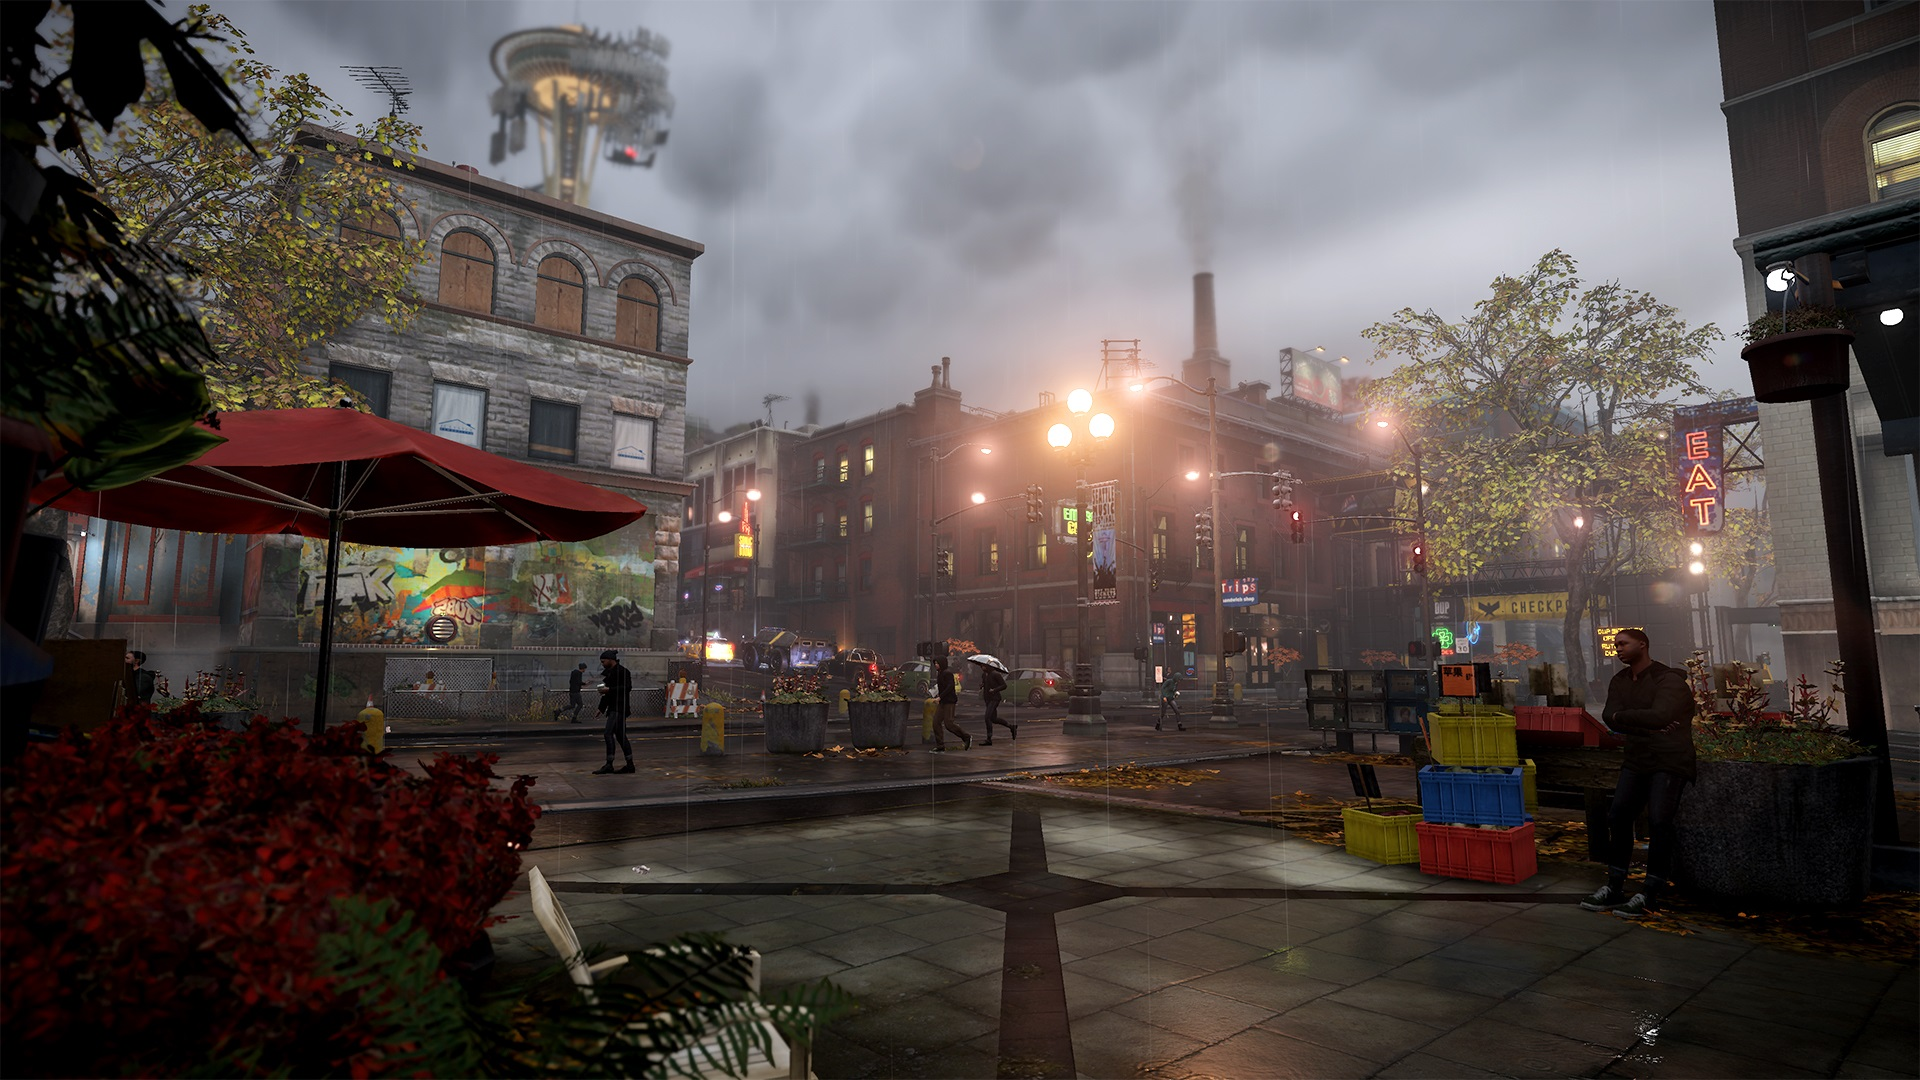
\includegraphics[width=\linewidth]{imagens/cidade_1.jpg}
\end{figure*}

\subsection{\bf História}
Os seres humanos sobreviveram ao Apocalipse por puro "milagre", diversas cidades foram destruídas, florestas queimadas, durante a guerra as armas que foram utilizadas foram suficientes para transformar montanhas em pó, rios e lagos escureceram de cinza e sangue, a radiação que se espalhou pela terra, ar e o que sobrou de água acabou por exterminar boa parte da vida na terra.

O milagre que salvou os humanos chama-se Dominus Corporation, uma empresa que estava estudando um novo material resistente de aparência semelhante a um acrílico para construir bolhas de proteção contra a poluição que o mundo estava sofrendo, pouco antes da guerra essa empresa cresceu consideravelmente e devido a esse crescimento, pode adquirir orçamento suficiente para concluir suas pesquisas e desenvolver a Nephila, com ela foi possível construir algumas cidades Colmeia, como são chamadas, são cidades envoltas num domo de proteção, onde a poluição de fora não consegue penetrar. Nas colmeias a vida continua aparentemente normal, como se o apocalipse nunca tivesse acontecido, as pessoas trabalham, estudam e seguem suas rotinas, a única obrigação é que eles devem tomar algumas pílulas de proteção contra a radiação e passar por exames anuais, pois nada nunca mais vai estar 100\% seguro.

A guerra acabou e o véu foi rasgado, hoje em dia existem mais pessoas dispostas a caçar o sobrenatural do que nos tempos antigos, se um Garou for visto perambulando pelas ruas, ele vai ser tratado como um monstro que merece ser executado, sua cabeça é tão premiada que em uma noite facilmente se juntaria 100 civis e uns 20 caçadores fortemente armados para abater a criatura, só para que assim possam ganhar um pouco de dinheiro vendendo seus restos.

\newpage
\begin{multicols}{2}

\subsection{\bf Cenário}
\imgColuna{imagens/cidade_2.jpg}
\subparagraph*{Colmeias são cidades protegidas com a tecnologia da Dominus Corporation, de formato circular, nelas foram construídos diversos arranha-céus, os mais bem equipados e melhores no geral ficam próximos ao centro, enquanto as “favelas em pé” ficam localizados as margens da colmeia, estas construções foram feitas com o que sobrou dos recursos do mundo e o que sobrou de melhor ficou para os ricos e poderosos. Uma curiosidade sobre os arranha-céus é que sempre o maior deles é chamado de Palácio, sempre localizado no centro da cidade e é comandado por uma Rainha. O clima dentro das colmeias é sempre quente, coisa de 35º com uma variação pequena para mais ou para menos. De dentro da Colmeia não é possível enxergar o mundo exterior.}

\imgColunaLegenda{imagens/cidade.jpg}{Cidade e seus Setores}
\subparagraph*{As cidades são sempre bem protegidas, existem patrulhas de policiais continuamente, a fim de evitar quaisquer conflitos que surjam dentro da Colmeia, afinal de contas, as pessoas precisam sempre obedecer às regras impostas pelas Rainhas.
As colmeias se ligam por meio de túneis subterrâneos, totalmente desconhecidos pela população comum, somente os responsáveis pela preservação destes túneis detêm conhecimento sobre os mesmos. Estes túneis são protegidos por soldados fortemente armados e as vezes por algumas criaturas desconhecidas.}
 
\subsection{\bf Habitantes do Setor 0}
\imgColuna{imagens/civis.jpg}
\subparagraph*{No setor 0 existem o que chamam de "Favelas" são prédios gigantescos com seus 100 andares e seus $4km^2$. Neste setor existe todos os tipos de miseraveis, pessoas simples em que seus antepassados não possuiam influência suficiente para garantir uma boa morádia nesse novo mundo.}
\preencher

\subsection{\bf Penumbra}
\imgColuna{imagens/penumbra.jpg}
\subparagraph*{A visibilidade na penumbra é sempre precária, existe somente a luminosidade de uma pequena luz que é emitida ao alto do domo, que dá um tom avermelhado ao ambiente. Ela também possui climas extremos, durante o dia a o ar é muito denso e quente, a temperatura chega facilmente aos 40º, a dor e o sofrimento é palpável no odor repugnante que exala de cada rua e buraco que possa ser encontrado, é possível sentir o sofrimento de forma intrínseca. A partir das 16 horas o clima muda abruptamente, a temperatura que antes estava em torno dos 40º facilmente vai abaixo dos -10º, os espiritos que se debatiam agora são congelados e ficam totalmente imóveis para que as aranhas possam vir se alimentar deles, elas adquiriram o habito e a habilidade de sugar a essência destes sem que morram, fechando a ferida com uma substância amarela que escretam de suas quelíceras.}

\subsubsection{\bf Espiritos}
\imgColuna{imagens/espirito_torturado.jpg}
\subparagraph*{Ao caminhar pela penumbra das colméias é possível ver espíritos moribundos presos a teias enegrecidas ou avermelhadas, alguns destes com olhares apáticos e vázios que seguem os viajntes livres, enquanto há outros ensandecidos, que se debatem de forma lenta, como se já estivessem cansados de lutar, mas que ainda não desistiram, mas é perceptível que a maioria perdeu sua essência.}

\newpage
\subsection{\bf Aliados}
\subsubsection{\bf Ían - Fianna, Philodox}
\imgColunaLegenda{imagens/ian.jpg}{Ían - Fianna, Philodox}
\subparagraph*{Rapaz calmo e sereno, possui uma paixão incontrolável por sua esposa Wanessa. Tornou-se líder do grupo de resistência Dominus não por vontade própria, mas por escolha dos que o seguiam. É extremamente brincalhão em alguns momentos e em outros parece sofrer de uma tristeza imensurável.}
\preencher

\subsubsection{\bf Hans Hughes-Becker - Parente Senhor das Sombras}
\imgColunaLegendaTexto{imagens/hans.jpg}{Hans - Parente Senhor das Sombras}
\subparagraph*{A sagacidade e esperteza de Hans é surpreendente, um rapaz bonito, se veste bem, fala bem e suas palavras sempre trazem algo escondido, ele sabe usar tudo a seu alcance para atingir seus objetivos, protetor fervoroso de sua irmã a Hanna. Hans já fez de tudo para sobreviver na colmeia, desde roubo, tráfico, até chegou ao ponto de se prostituir por algumas noites para não ver sua irmã passar fome. É amargurado por diversos motivos, mas principalmente por não ter conseguido se transformar na forma completa de batalha, a Crinos, mas tem total controle da forma Glabro.}
\preencher

\subsubsection{\bf Hanna Hughes-Becker - Senhora das Sombras, Ahroun}
\imgColunaLegenda{imagens/hanna.jpg}{Hanna - Senhora das Sombras, Ahroun}
\subparagraph*{Uma moça bonita, que não consegue esconder sua antiga paixão por Ían, mesmo sabendo que ele já é compromissado com Wanessa. Hanna possui um cabelo curto pintado de loiro, suas vestes demonstram sua personalidade rebelde e seu jeito é sempre debochado, ela sempre se acha superior aos seus rivais, seja em combate ou no amor.}
\preencher


\subsubsection{\bf Domic “Dom” Olsen - Cria de Fenrir, Theurge}
\imgColunaLegenda{imagens/dom.jpg}{Dom - Cria de Fenrir, Theurge}
\subparagraph*{Rapaz sério, muito apegado a seus bens e grande profissional, já fez de tudo na vida, desde carpintaria, pintura, até furtos nas ruas, é moreno cabelo curto quase careca, possui braços mecânicos que ele mesmo fez. Se esforça ao máximo para tentar ser simpático, mas não consegue, pois, coisas mínimas sempre o irritam.}
\preencher

\subsubsection{\bf Michael “Mike” Buford - Parente Peregrino Silencioso}
\imgColunaLegenda{imagens/mike.jpg}{Mike - Parente Peregrino Silencioso}
\subparagraph*{Rapaz simpático de 20 e poucos anos, com cerca de 1,80m de altura, cabelos pretos, lisos e curto, pele caramelo claro e de porte atlético magro. É um rapaz extremamente simpático e amigável, sonhador nato, seu principal objetivo é descobrir uma forma de sair das Colmeias e viver uma vida de verdade do lado de fora. É um parente com dons especiais, consegue levar pessoas já mais propensas a acreditarem no que ele diz, parece conseguir se comunicar com ancestrais do passado e possui grande conhecimento do que já foi a sociedade Garou.}
\preencher

\subsubsection{\bf Wanessa} 
\imgColunaLegenda{imagens/wanessa.jpg}{Wanessa - Parente}
\subparagraph*{}
\preencher


\subsection{\bf Abrigo}
\imgColunaLegenda{imagens/abrigo.jpg}{Esconderijo e Abrigo dos Aliados}

\subsection{\bf Antagonistas}
\subsubsection{\bf O Último Garra (Garras-de-Ossos)} – É o último Garou dos Garras Vermelhas, sobreviveu ao apocalipse de forma totalmente inesperada, ele viu seus companheiros serem massacrados pelos caçadores durante o apocalipse e isso só fez aumentar ainda mais seu ódio pelos humanos, o fazendo chegar ao ponto de aceitar a corrupção da Wyrm. É um lupino extremamente forte e sagaz, com a experiência de um ancião, infelizmente pela sua queda a Wyrm ele se tornou o líder de uma matilha de espirais, os nomeando de “Profanadores da Carne”, cujo único objetivo é caçar, matar e destruir tudo que já foi tocado pelo homem. Seu augúrio é desconhecido, mas é bem provável que ele detenha os dons de todos os augúrios.

\subsubsection{\bf Maeve R. Copehan} – Rainha que controla a colmeia, mulher com uma beleza sobrenatural, sorriso estonteante, palavras doces e atitudes cruéis, ela pode muito bem mandar uma família inteira para fora da colmeia simplesmente por estes não terem uma foto sua em um pedestal em suas tão “milagrosas” casas, ou qualquer coisa fútil do tipo. É exatamente o tipo de pessoa que você não quer ter por perto ou quer que saiba de sua existência, pois ela pode não ir com sua cara pelo simples fato de você existir.

\subsubsection{\bf Doutor Arthur VanDerVart} – Geneticista chefe da Dominus, é responsável por todo avanço da tecnologia contra os garou, foi quem descobriu como inibir o sangue e impedir a primeira transformação. Também chefiou os cientistas na criação das quimeras, os "garou" criados a partir do sangue de impuros e atualmente está trabalhando em um projeto ainda secreto. É um dançarino da pele, ele aprendeu como fazer para se tornar um Garou por completo, só que aliou a tecnologia, ciência e misticismo para amplificar o poder do ritual, alguns dizem que ele utilizou das peles dos garou mais poderosos para montar seu manto.

\subsubsection{\bf Sussurros-do-Abismo} -  um espirito extremamente poderoso, utiliza de seus cantos e performance como formas de rituais para sugar a alma de seus seguidores, já existe a séculos, mas só agora ele mostrou sua verdadeira face, era um simples espirito da Weaver, mas conseguiu assimilar diversos espíritos da Wyrm e da Wyld com seus cantos. Não se deve dar ouvidos a ele. É um espirito imponente, quando canta sua respiração é pesada e sua voz imperiosa é semelhante a um cântico em coro. Em tamanho ele tem cerca de 1,90m, sua forma é humanoide e um tanto robusta, possui 4 braços e uma máscara que tampa seu rosto quase que completamente, deixa apenas seus olhos de fora e o que se pode perceber é que tem uma pele avermelhada e olhos profundos, como se estivesse enxergando sua alma. Ele procura sempre tomar formas semelhantes a grandes cantores e segue tendências musicais que trazem facilidade a seus encantos. 

\subsubsection{\bf Caçadores} 
\imgColunaLegenda{imagens/cacadores.jpg}{Os mercenários}
\subparagraph*{Autoentitulados \textit{caçadores}, estes mercenários habitam todo o Setor 0 e possuem uma rede extensa de informantes e um arsenal especializado em matar criaturas sobrenaturais. Como já não encontram mais as criaturas os caçadores se voltaram contra a população e buscam por qualquer pessoa que tenha sua foto colocada num cartaz de procurado ou que possa ter algum envolvimento com as criaturas.}
\preencher

\subsubsection{\bf Juízes} 
\imgColunaLegenda{imagens/juiz.jpg}{Policiais de Elite}
\subparagraph*{Os policiais são conhecidos como Juízes, andam sempre em grupos, fortemente armados e com ordem para conter a todo custo, qualquer transgressão as leis da Rainha. Eles podem não saber, mas suas armas são fetiches da Weaver com espíritos da tecnologia neles, porém os espíritos foram obrigados a entrar na arma e quando estas são ativadas, a gnose do espirito é sugada brutalmente até causar a morte deste.}
\subsection{\bf Sistema}
\subparagraph{\bf População de Garou:} Desconhecida.
\subparagraph{\bf Quantidade de Caerns:} 0.

\subsubsection{\bf Limitações de criação de ficha}
\begin{enumerate}
\item Somente permitido jogar com hominídeo;
\item Não pode ter raça pura, nem totem;
\item Não pode ter nenhum antecedente acima de 3;
\item Não pode possuir nenhuma habilidade acima de 3 pontos pois o 4º ponto será ganho automático em um momento do jogo;
\item Não é permitido força de vontade, gnose ou fúria acima de 6 pontos;
\item Não pode pegar nenhuma qualidade ou defeito que deixe suspeita sobre sua vida garou, pois o mundo caça impiedosamente os que são “parecidos” com lobos, semelhante a época da inquisição e da caça às bruxas;
\item Somente é possível gastar 3 pontos de bônus em habilidades secundárias (equivalentes a 6 pontos totais);
\item Atributos só podem possuir uma especialização por característica;
\item Andarilhos do Asfalto recebem um bônus de +2 dados quando o teste envolver coisas tecnológicas;
\end{enumerate}

\subparagraph{\bf As Tribos}
As tribos que sobraram é um amalgama de Andarilhos do Asfalto com as restantes, o mundo ficou muito tecnológico para as tribos ficarem para trás.
\begin{enumerate}
\item Garras Vermelhas, Wendigo, Fúrias Negras (extintas);
\item Uktena (desaparecida);
\item Presas de Prata, Portador da Luz Interior, Filhos de Gaia, Peregrinos Silenciosos (próximas da extinção);
\item Fianna, Crias de Fenrir, Senhores das Sombras (existem poucos);
\item Andarilhos do Asfalto, Roedores de Ossos (os mais numerosos em comparação aos restantes);

\item [*] Quando digo extintas significa que não são jogáveis,porém é possível adquirir seus dons com um custo de 4x nível do dom se for bem explicado a forma de se adquiri-lo.
\item [**] Quando digo próximas da extinção, significa que ainda não são jogáveis no início da crônica, mas é provável que se encontre alguns deles por aí. Em relação aos dons é semelhante ao caso da extinção.
\item [***] Desaparecido está totalmente sumido, não se sabe o paradeiro dos mesmos, se estão extintos ou escondidos. 
\item [****] Devido as limitações de raças, os dons delas podem ser adquiridos como dons de hominídeos, se for conseguido explicar como funcionam em você e porque você o tem.
\item [*****] Mesmo sendo um amalgama de Andarilhos, somente será permitido pegar os dons deles como se fossem seus tribais até o nível 2.
\end{enumerate}

\subparagraph{\bf Custos de Experiência (XP)}
O gasto de experiência segue a seguinte configuração:
\begin{itemize}
    \item Dons de hominídeo/tribo/augúrio: 3 x nível
    \item Dons de outras raças/tribos perdidas: 4 x nível
    \item Dons de outras tribos: 5 x nível
\end{itemize}

\subsubsection{\bf Totens}
\subparagraph{\bf Skoll:} 
\imgColunaLegenda{imagens/skoll.jpg}{Skoll, O Grande Lobo}
\subparagraph*{Skoll, um dos filhos do Grande Fenrir se manteve vivo nesses tempos, aprisionado como seu patrono, ele se manteve firme ao resistir a prisão que as aranhas do padrão o haviam colocado, mesmo fraco com o passar dos anos se recusou a ceder sua vida para as feras metalicas que habitavam a penumbra da colméia.
Ele é um lobo imenso, chega facilmente aos 4m de altura, sua pelagem negra e glifos vermelhos em brasa deixam bem claro do porque ele era conhecido como a personificação da Fúria.
Skoll foi aprisionado nas teias do padrão, em meio aos climas extremos da penumbra, sendo vigiado continuamente por 4 aranhas do padrão.}

\subparagraph*{\bf Descrição:} Skoll fica mais forte conforme sua ligação com a matilha aumenta, a cada determinado nível atingido ele permite que seus protegidos utilizem de alguns de suas habilidades e encantos.
\begin{itemize}
    \item Nível 10: Armadura de Luna
    \item Nível 13:
    \item Nível 15: Espirito de Batalha
    \item Nível 17: 2 encantos a escolha dos jogadores
    \item Nível 20: +1 dado em todo teste envolvendo combate
\end{itemize}
\subparagraph*{\bf Bônus:} 1 de destreza, 1 de prontidão, 1 de esquiva, 1 de furtividade, 1 de gnose.
\subparagraph*{\bf Caracteristicas:}
Fúria 8, Gnose 5, Força de Vontade 7, Essência 21.

\subparagraph{\bf Hati:} 
\imgColunaLegenda{imagens/hati.jpg}{Hati, A Alfa}
\subparagraph*{Hati, assim como seu irmão Skoll, é uma dos filhos do Grande Fenrir, ela estava desaparecida até que foi feito o ritual do "Lobo Adormecido", onde é preciso o sacrificio de um lobo e um Garou, para que o espirito possa reecarnar. Hati é a personificação da serenidade e do equilibrio com o mundo espiritual, ao contrário do seu irmão.}
\subsection{\bf Dossiê}
\begin{itemize}
    \item Garras Vermelhas – Os mais selvagens dos garous lutaram bravamente, mas seus poucos números logo foram dizimados quando as hordas da Wyrm atingiram seus Caerns, espalhando destruição e poluição.
    \item Fúrias Negras – As mais próximas da Wyld sofreram ao tentar combater com toda sua fúria, não tiveram a mesma sorte dos Crias, mas ainda assim levaram consigo um número incontável de dançarinos da espiral.
    \item Wendigo – O povo puro foi o primeiro a sofrer com as armas químicas utilizada na guerra, eles não tiveram força e nem sequer formas de se defender da onda de calor e radiação que surgiu ao horizonte a explosão das bombas.
    \item Uktenas – Partiram em missões onde acabaram descobrindo um ritual de proteção muito poderoso, chamado de "O Lobo adormecido", a tribo ficou por muito tempo na umbra em busca desse conhecimento e pagou um preço alto demais ao executar o ritual, este foi realizado com sucesso, mas desde então não se vê mais sinais dos Uktena.
    \item Peregrinos Silencios – Foram os primeiros a reagirem ao apocalipse, até porque começou em uma terra que já foi sua, com o despertar de um deus servo da Wyrm, que utilizou de um garou puro para seu ritual de levantar dos mortos.
    \item Filhos de Gaia – A vontade de tentar purificar seus irmãos caídos sob o feitiço do deus, fez com que os Filhos de Gaia perdessem muito tempo e ficassem muito próximos a podridão, infelizmente eles não conseguiram resistir e acabaram por ser massacrados.
    \item Presas de Prata – Os líderes da nação demoraram a agir e acabaram por tomar o primeiro ataque, lutaram em todas as batalhas liderando as tropas contra os inimigos, mas não tiveram sucesso, os remanescentes caíram em harano e desapareceram, seu sangue puro e nobre foi caçado no novo mundo.
    \item Portadores da Luz Interior – Devido a sua luta para proteger os montes sagrados os portadores da luz não tiveram muitas chances de sobreviver, não se sabe se ainda exista algum deles por.
    \item Fianna – Os melhores amigos da nação e os mais ligados a seus parentes, tiveram perdas imensas na guerra, mas sua grande prole de parentes permaneceu firme no novo mundo.
    \item Crias de Fenrir – Os guerreiros dos guerreiros, eles foram um dos primeiros a se manifestar quando o apocalipse teve início. Partiram para o combate sem conhecimento do que era de fato e acabaram por perder diversos irmãos de garra, quando notaram do que se tratava se aliaram aos Fianna e aos Presas de Prata para tentarem fazer frente a guerra que havia começado. Devido a sua força física incomparável, eles conseguiram se manter por algum tempo, mas somente seus parentes foram capazes de sobreviver no novo mundo.
    \item Senhores das Sombras – Os métodos exclusos dos senhores das sombras os deram uma dianteira frente a criação da nova sociedade, seus parentes, aliados e contatos facilitou a entrada deles no novo mundo, a falta de escrúpulos também os ajudou a manter as aparências.
    \item Roedores de Ossos – Os roedores por serem mais próximos aos humanos conseguiram propagar seus genes através dos parentes, que foram se camuflando em meio a nova sociedade. Devido a sua facilidade de sobreviver em meio a adversidade eles não tiveram muitos problemas em sobreviver sendo os miseráveis do novo mundo, até porque já eram os miseráveis do antigo.
    \item Andarilhos do Asfalto – A aproximação com a tecnologia trouxe uma enorme vantagem aos Andarilhos, pois eles puderam prever os acontecimentos do meio tecnológico e rapidamente se inseriram no início da criação das colmeias, garantido sua vaga na nova sociedade que se instaurou.
\end{itemize}

\subsection{\bf Apêndice}
\subparagraph{\bf Fetiches:}

\subparagraph{\bf Glossário:}
\begin{enumerate}
    \item {Dominus Corporation}: A empresa que comanda todas as colmeias, aliada a Weaver no mundo físico e encarregada de tecer a película pelo mundo físico.
    
    \item {Nephila}: Nome dado ao material utilizado na criação das colmeias, muito resistentes superando em muito o aço e até mesmo a resistência dos dentes de alguns moluscos.
    
    \item Palácio: Sempre localizado no centro das Colmeias e é onde ficam as “Rainhas”
    
    \item Rainha: Governante responsável pelo controle das colmeias, sempre são mulheres.
    
    \item Quimeras: As criaturas que guardam os túneis são mutantes desenvolvidos por filiais da Dominus, são “garou” criados a partir do sangue de impuros e que sofreram uma mutação genética, são extremamente agressivos.
    
    \item O Lobo Adormecido – Ritual de proteção, elaborado por Luna e os Uktena para proteger os parentes dos garou de forma a serem mais difíceis de serem detectados pelos espíritos da Weaver e Wyrm, o ritual possuí um tempo limite e parece que o tempo está se esgotando. 
\end{enumerate}
\end{multicols}
\imgFundoTexto{litania.png}{

\vspace{-40pt}

\Huge \titulo{A Litania}

\parskip=18pt

\begin{center}
\huge \bf \it
Não te Acasalarás Com Outro Garou.

Combaterás a Wyrm Onde Ela Estiver e Sempre Que Proliferar.

Respeita o Território do Próximo.

Aceita uma Rendição Honrosa.

Submete-se aos Garou de Posto Mais Elevado.

Oferece o Primeiro Quinhão da Matança aos de Posto Mais Elevado.

Não Provarás da Carne Humana.

Respeita Aqueles Inferiores a Ti: Todos Pertencem a Gaia.

Não Erguerás o Véu.

Não Serás um Fardo Para Teu Povo.

Não Desafiarás o Líder em Tempos de Guerra.

Pode-se Desafiar o Líder em Tempos de Paz.

Não Tomarás Qualquer Atitude Que Provoque a Violação de um Caern.

\end{center}
}

\imgFundo{fundo.jpg}

%\begin{pycode}
%\end{pycode}

\end{document}